\chapter{Umsetzung}

In diesem Kapitel werden die technischen Hintergründe der einzelnen Komponenten erläutert und ihre Umsetzung beschrieben.
....


\section{Motoransteuerung}

Eine Motorsteuerung ist nötig um die Geschwindigkeit eines Motors einstellen zu können. Dem Auto liegt ab Werk bereits ein Motortreiber bei,
welcher genau diese Funktion übernehmen kann. Im folgenden Abschnitt wird beschrieben, warum dieser nicht genutzt werden kann und wie die Lösung aussieht.

\subsection{Treiberbausteine}
Da die gewählten Akkus eine Spannung von 14,4V aufweisen, kann der original Motortreiber leider nicht verwendet werden.
Denn dieser benötig eine Spannung von 7,4V. Da der AVR Mikrokontroller mit 5V betrieben wird, wird ein Motortreiber benötig der
mit den 5V Pegeln arbeiten kann. In vielen Mikrocontroller-Projekten und in unserem ersten Prototyp wird der ``L298 DUAL FULL-BRIDGE DRIVER''
verwendet. Dieser ist leider auch bei der Benutzung beider Kanäle auf 4 Ampere begrenzt \cite{L298}, was beim Prototyp zu einer permanenten
Überlastung des Treibers führt. Die benötigte maximale Belastbarkeit des Motortreibers wurde in einem kurzen Expriment ermittelt 
und beträgt 20 A. Leider sind keine vollintegrierten Motortreiber mit der benötigten Belastbarkeit verfügbar. 
Eine Möglichkeit dieses Problem zu umgehen und unseren Anforderungen, wie Vor- und Rückwärtsbetrieb, zu genügen  
wird ein Vierquadrantensteller aus diskreten Mosfets aufgebaut.

\subsubsection{Vierquadrantensteller}
Definition nach Wikipedia\cite{vierquadrantensteller}:\\
``Ein Vierquadrantensteller besteht aus einer elektronischen H-Brückenschaltung aus vier Halbleiterschaltern, meist aus Transistoren, 
welche eine Gleichspannung in eine Wechselspannung variabler Frequenz und variabler Pulsbreite umwandeln kann. Vierquadrantensteller 
in der Energietechnik können auch Wechselspannungen unterschiedlicher Frequenzen in beiden Richtungen ineinander umwandeln.''


\begin{figure}[H]
\centering
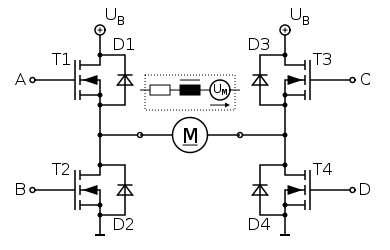
\includegraphics[width=.8\textwidth]{Vierquadrantensteller.png}\\
\caption{Vierquadrantensteller \cite{vierquadrantensteller}}%
\label{fig:Vierquadrantensteller}
\end{figure}


Auf Grund der hohen Belastbarkeit und leistungslosen Ansteuerung werden meist Mosfets als Halbleiterschalter genutzt. Um die beiden oberen Mosfets (T1/T3) durchzuschalten
ist auf Grund des fehlenden Massepotentials eine Gatespannung oberhalb der Betriebsspannung nötig. Diese wird meist mittels Bootstrapping zur
Verfügung gestellt. Da das simultane Durchschalten der übereinander liegenden Mosfets zu einem Kurzschluss führen würde, muss dies durch
eine Schutzschalung verhindert werden. Um all diese Funktionen zur Verfügung zu stellen gibt es bereits fertige Mosfettreiber,
welche das Schaltungsdesign enorm vereinfachen.


\subsection{Mosfets}
Als geeignete Mosfets wurden die FDD6690A von Fairchild Semiconductor ausgewählt. Diese sind zugelassen bis zu einer Drain-Source-Spannung von 30V und einer maximalen Dauerbelastung
von 46A, eine gute Kühlung vorausgesetzt. Des Weiteren verfügen sie über einen sehr niedrigen Drain-Source-Widerstand von $R_{\text{DS(ON)}}= 12 m$, was zu einer niedrigen Verlustleistung führt. Durch ihre niedrige 
Gate Ladung von 13nC eignen sie sich gut für hohe Schaltfrequenzen. Auf Grund dieser Eigenschaften sind sie hervorragend für einen Motortreiber geeignet.


\subsection{Mosfettreiber}
\subsubsection{Verfügbarkeit}

Mosfettreiber gibt es in vielen Ausführungen, unter anderem als ``Single Channel High Side Driver``, ``Half Bridge Driver'', ``Full Bridge Driver''
und ``3 Phase Driver''. Da für den verbauten DC-Motor eine Vollbrücke nötig ist, um den Motor in alle Richtungen zu betreiben, werden an dieser Stelle
ausschließlich ``Full Bridge Driver'' untersucht.

Eine Tabelle auf Mikrocontroller.net\cite{FET_D_TABLE} zeigt eine Auswahl an verfügbaren Mosfettreibern. Dort sind zwei
``Full Bridge Driver'' aufgeführt, welche für dieses Projekt passend sind. Allerdings fällt die Entscheidung auf einen anderen Treiber,
dem Allegro A3941.
\subsubsection{Allegro A3941}
Der Allegro A3941 ist für Betriebsspannungen von 5,5V bis 50V geeignet und liegt damit in der Spezifikation des Projekts.
Des Weiteren verfügt der Motor über eine integrierten 5V Regulator und kann somit ohne Spannungsregulator am Akku betrieben werden.
Über zwei Ausgänge der Treibers können diverse Fehler ausgelesen werden. Auch sind alle gängigen Schutztschaltungen wie z.B. ein Kurzschlussschutz enthalten.


Der Treiber lässt sich in verschiedennen Modi betreiben:

\begin{figure}[H]
\centering
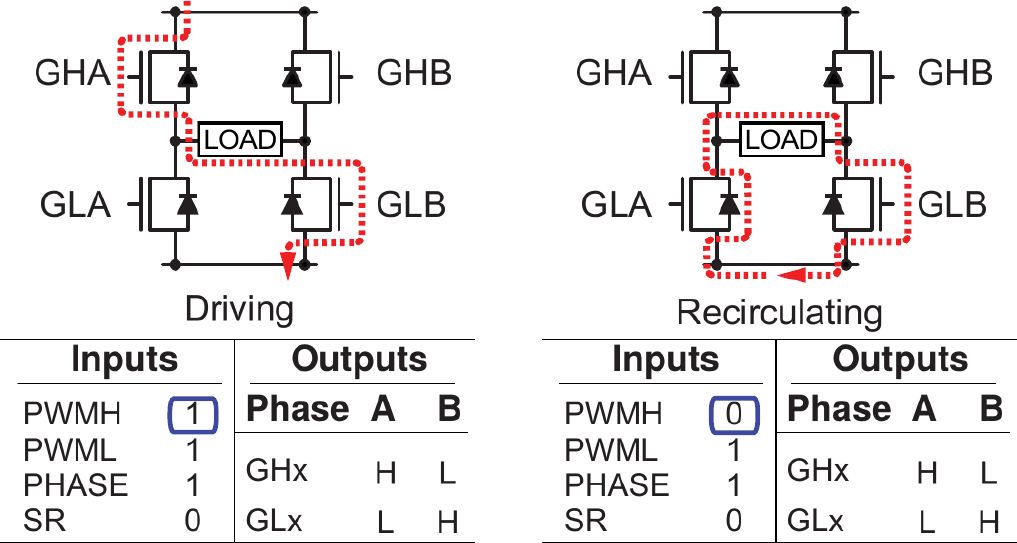
\includegraphics[width=.8\textwidth]{3941_1.png}\\
\caption{Slow decay, diode recirculation, high-side PWM \cite{ds-A3941}}%
\label{fig:39411}
\end{figure}

Konfiguration: PWML=1, PHASE=1, SR=0 und PWM an PWMH (high-side PWM)\\
Bei aktivierten PWMH fließt der Strom durch den GHA-Mosfets über den Motor und
dann über den GLB-Mosfet. in diesem Modus wird der Motor angetrieben.
Wenn PWML deaktiviert ist zirkuliert der vom Motor induziert Strom durch GLB und durch
die interne Diode von GLA, der Motor wird dadurch gebremst.


\begin{figure}[H]
\centering
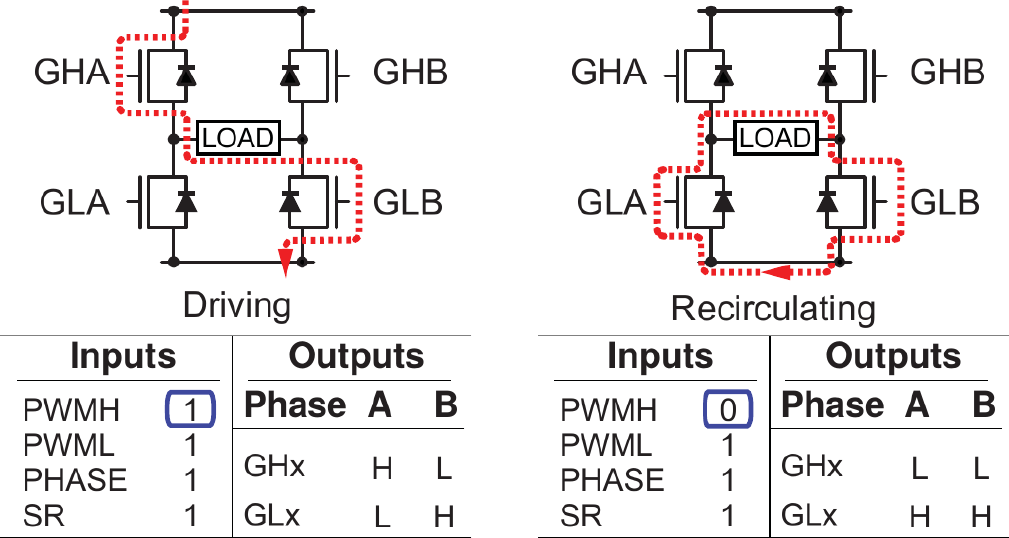
\includegraphics[width=.8\textwidth]{3941_2.png}\\
\caption{Slow decay, SR active, high-side PWM \cite{ds-A3941}}%
\label{fig:39412}
\end{figure}

Konfiguration: PWML=1, PHASE=1, SR=1 und PWM an PWMH (high-side PWM)\\
Bei aktivierten PWMH fließt der Strom durch den GHA-Mosfets über den Motor und
dann über den GLB-Mosfet. In diesem Modus wird der Motor angetrieben.
Wenn PWML deaktiviert ist zirkuliert der vom Motor induziert Strom durch 
GLB und durch GLA, der Motor wird durch den niedrigeren Innenwiderstand des Mosfest 
stärker gebremst als in der voherigen Konfiguration. Dabei ist darauf zu achten, dass
beinahe die gesamte vom Motor induzierte Spannung über den beiden Mosfets (GLA/GLB) abfällt,
was zu einer starken Hitzeentwicklung führen kann.



\begin{figure}[H]
\centering
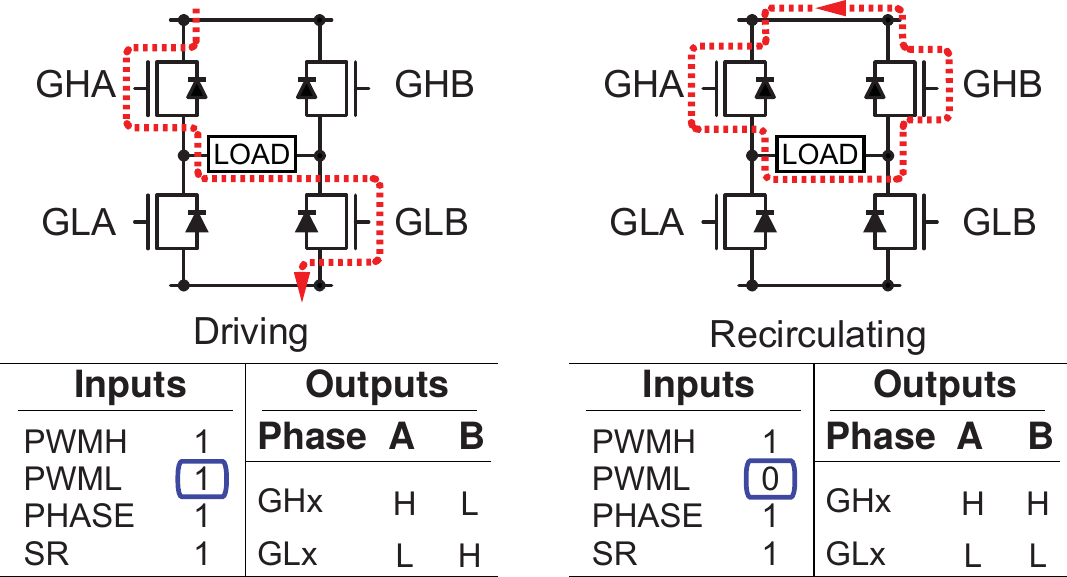
\includegraphics[width=.8\textwidth]{3941_3.png}\\
\caption{Slow decay, SR active, low-side PWM \cite{ds-A3941}}%
\label{fig:39413}
\end{figure}

Konfiguration: PWMH=1, PHASE=1, SR=1 und PWM an PWML (low-side PWM)\\
Diese Konfiguration entspricht im Grunde den beiden vorherigen, nur dass das PWM-Signal
an den unteren Mosfets anliegt. Der SR-Pin entscheidet wieder darüber ob im ``Bremsmodus''
die internen Dioden genutzt werden (SR=0) oder nicht (SR=1).




\begin{figure}[H]
\centering
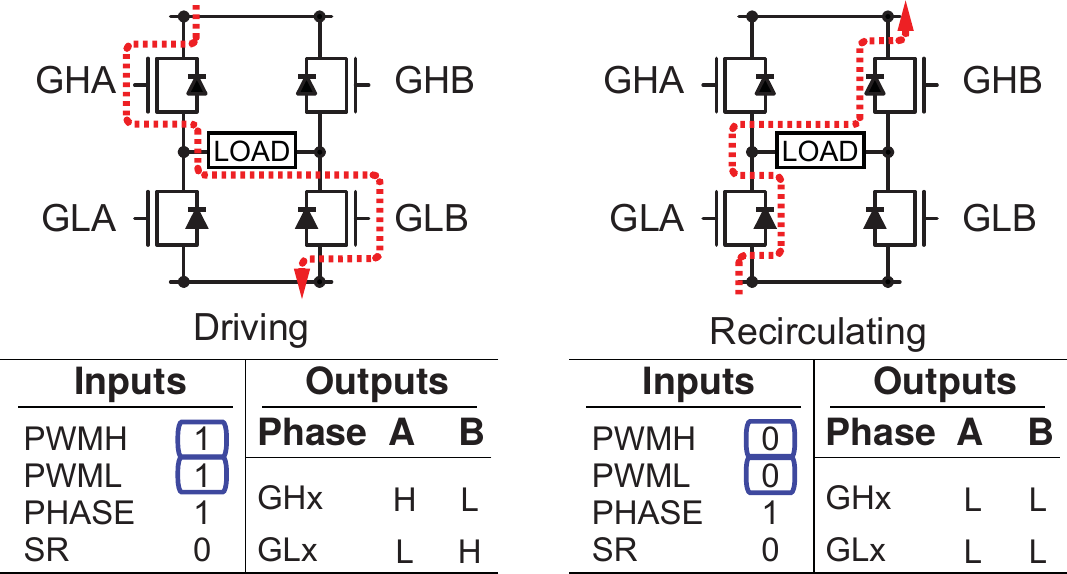
\includegraphics[width=.8\textwidth]{3941_4.png}\\
\caption{Fast decay, diode recirculation \cite{ds-A3941}}%
\label{fig:39414}
\end{figure}


Konfiguration: PWMH=1, PWML=1, PHASE=1, SR=1\\
In dieser Konfiguration werden die oberen und unteren Mosfets gleich geschaltet. Im
``Bremsmodus'' führt das dazu, dass der induzierte Motorstrom nicht über die Mosfets
zirkulieren kann. Der Strom fließt stattdessen zurück in die Spannungsquelle, was
abhängig von der Spannungsquelle zu Schäden führen kann. Wird die Schaltung jedoch an
einem geeigneten Akku betrieben, ist es so möglich die Energie zu nutzen und damit den Akku
zu laden.

\begin{figure}[H]
\centering
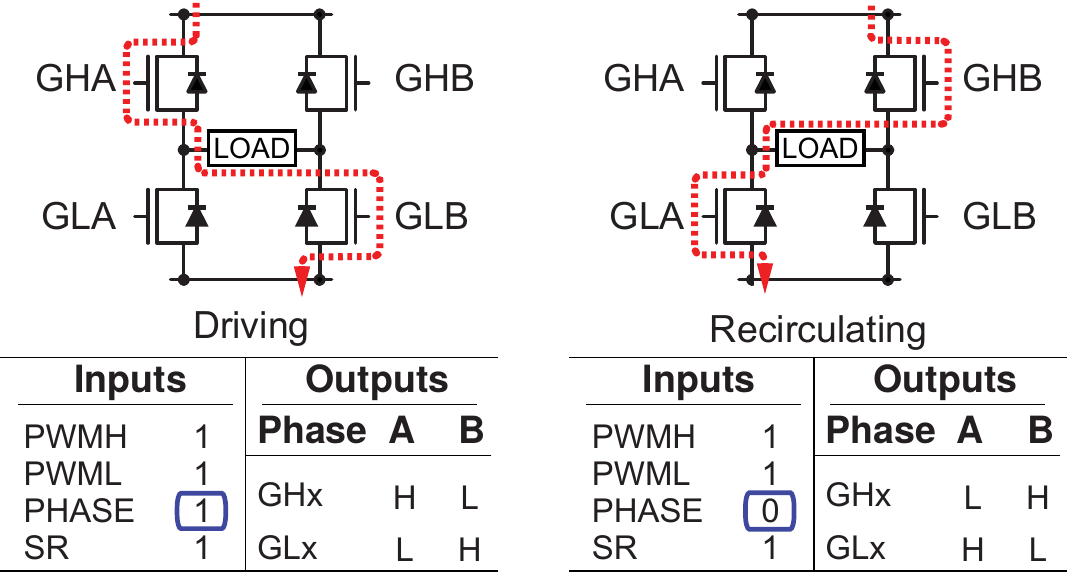
\includegraphics[width=.8\textwidth]{3941_5.png}\\
\caption{Fast decay, SR active, full four-quadrant control \cite{ds-A3941}}%
\label{fig:39415}
\end{figure}

Diese Konfiguration zeigt den Einfluss des PHASE-Pins. Liegt am PHASE-Pin 1 an
fließt der Strom von links nach rechts. Liegt 0 an fließt er von rechts nach links.
Mithilfe des PHASE-Pins wird also die Polung des Motors festgelegt.


\subsubsection{Schaltpan}

In Folgenden wird geklärt wie sich die Beschaltung des Allegro A3941 bestimmen lässt. Die Schaltung in \cref{fig:schalt:allegro} entspicht dabei den Vorgaben im Datenblatt.

\begin{figure}[H]
\centering
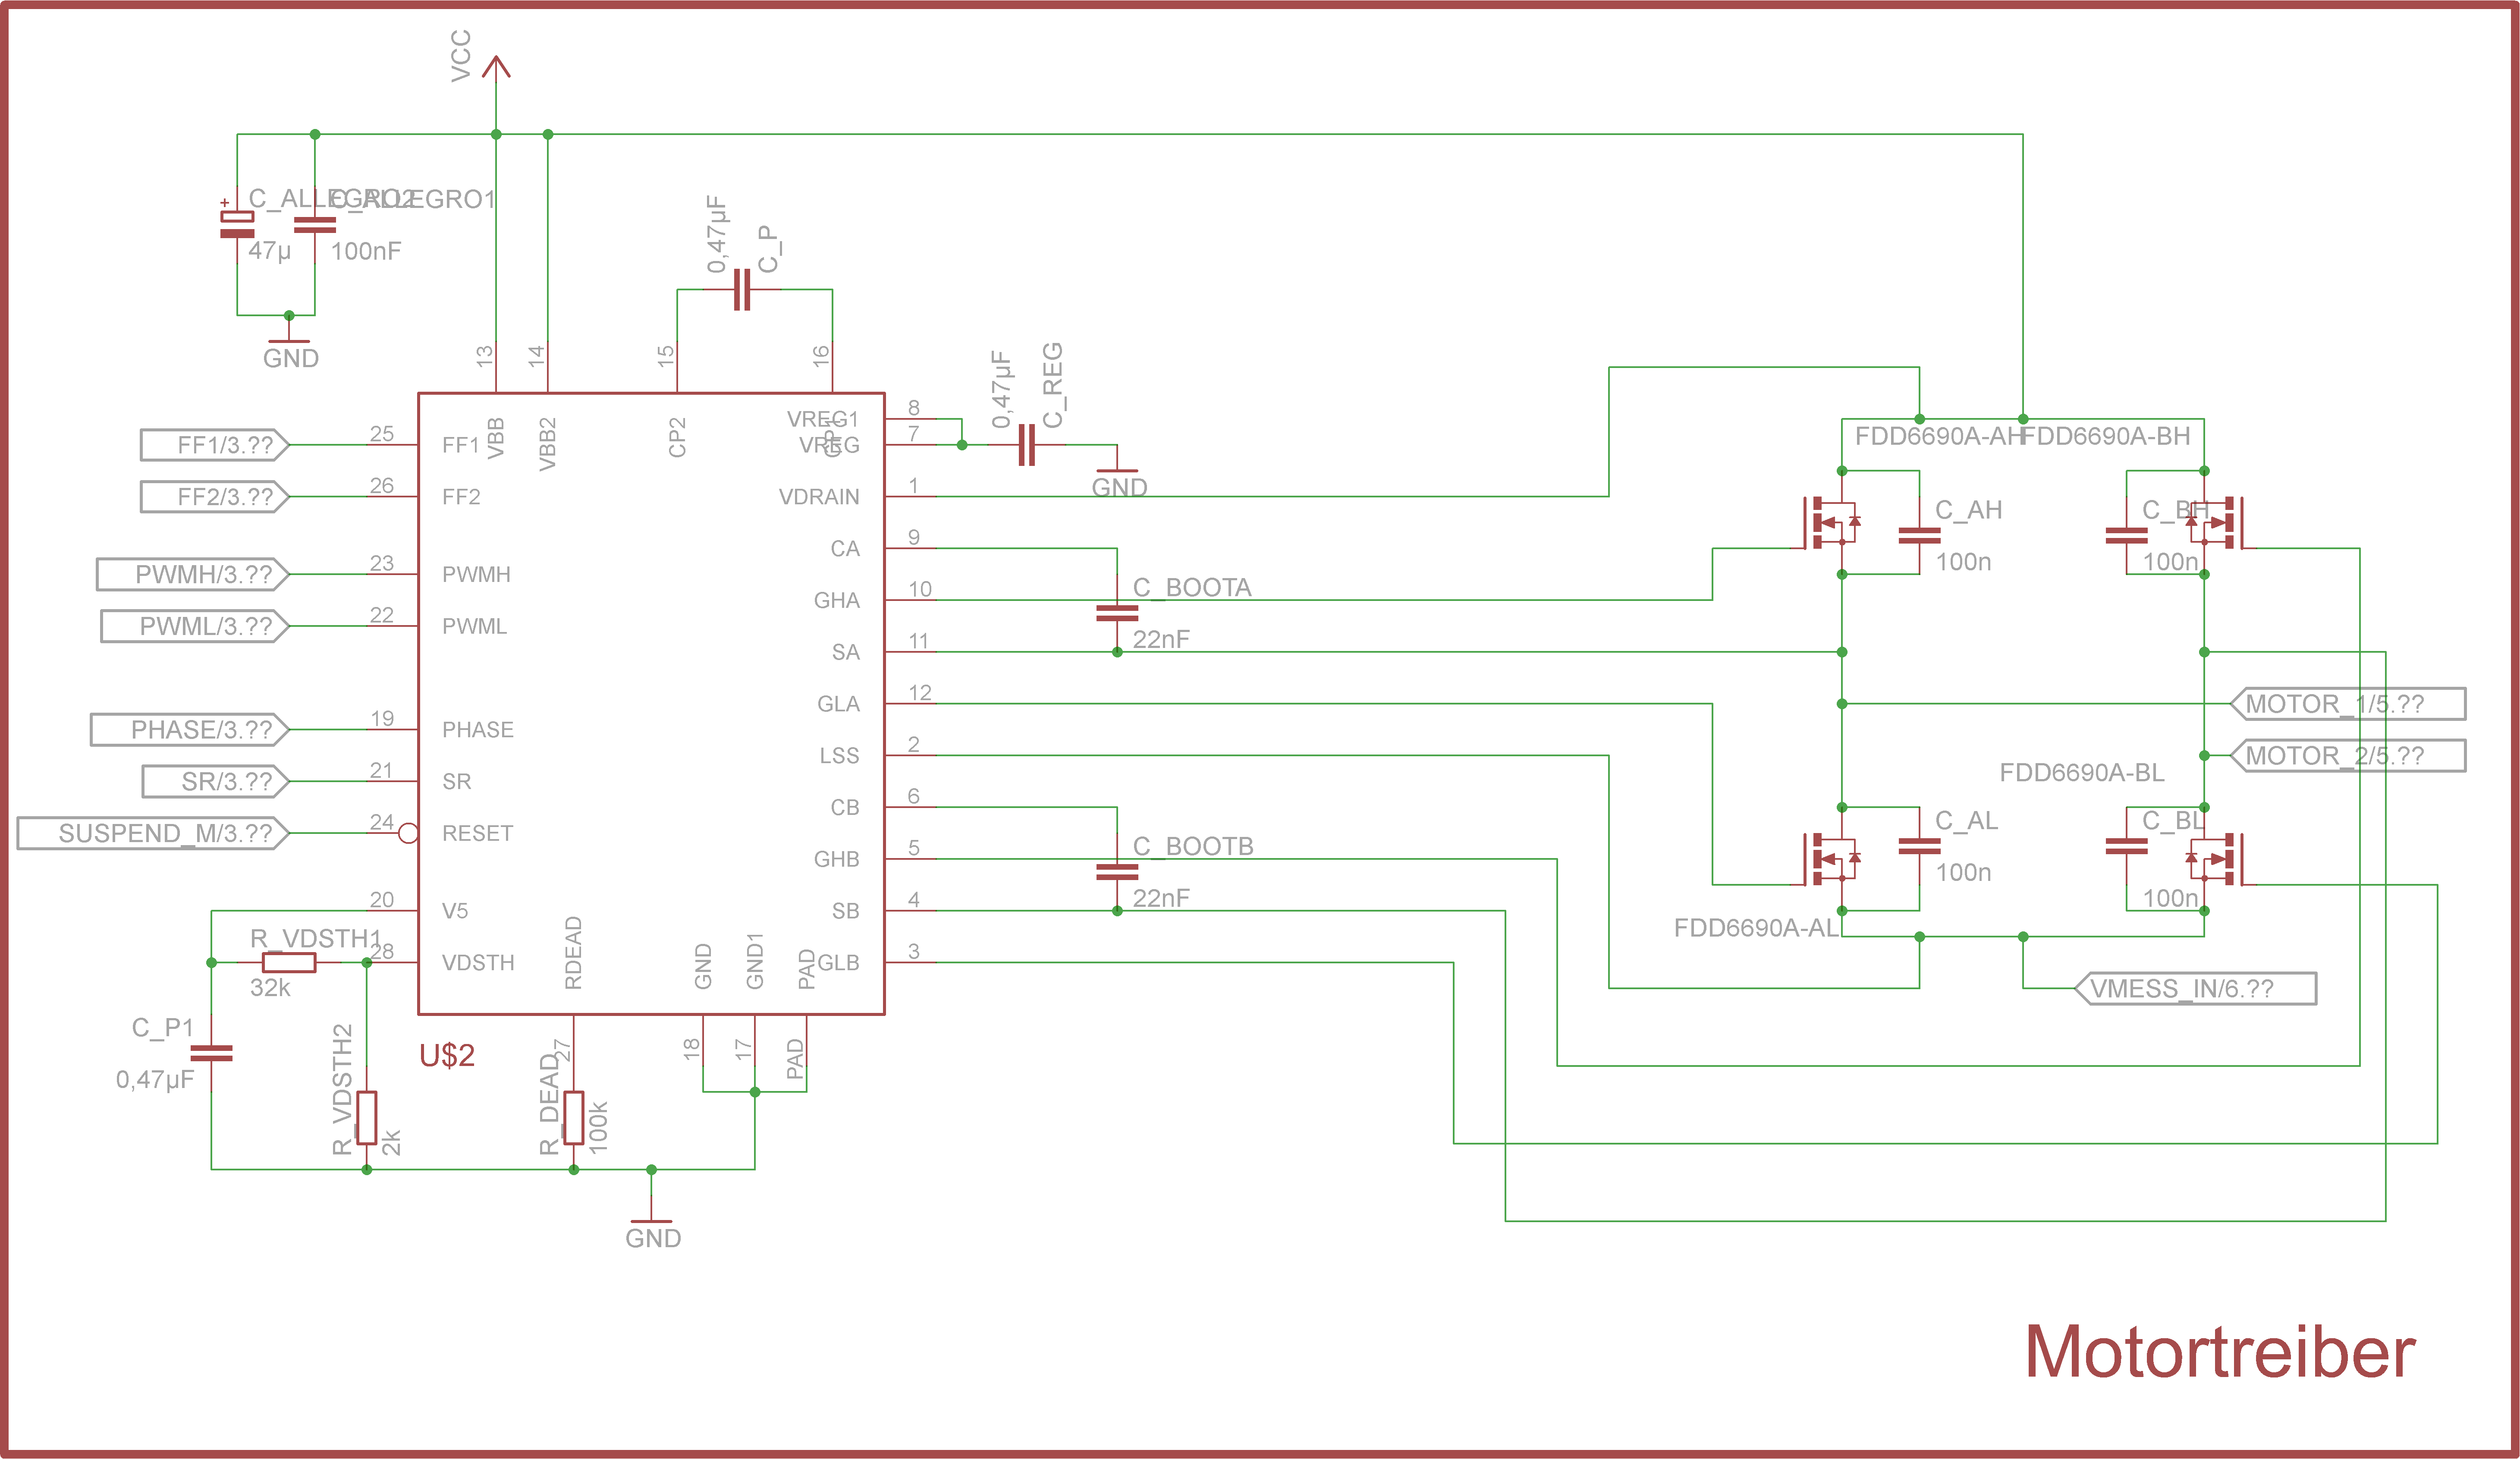
\includegraphics[width=.9\textwidth]{motortreiber.png}\\
\caption{Schaltplan Allegro A3941}%
\label{fig:schalt:allegro}
\end{figure}

$R_{\text{DEAD}}$ legt die Totzeit zwischen den Mosfetumschaltungen fest. Wird sie zu niedrig gewählt, können in jeder PWM-Periode Kurzschlüsse auftreten. Wird sie zu hoch
gewählt, beschränkt man das Tastverhältnis unnötig, was die Motorleistung reduziert. Da wir ``Low Gate Charge'' Mosfets nutzen, und die Einschalt- bzw. Ausschaltzeit
der Mosfets hauptsächlich von dieser Größe abhängt, ist diese Zeit sehr klein. Da jedoch eine genaue Bestimmung dieser Zeit für unseren Einsatz nicht nötig ist,
wird hier ein mittlerer Wert von $100k\Omega$ gewählt. Da sich dieser laut Datenblatt zwischen 3 und $240k\Omega$ befinden sollte.\\


%(ca 50ns).
%
% 
% Die Totzeit t\textsubscript{DEAT} bestimmt sich folgender Maßen (für 3-240k$\Omega$)
% 
% \begin{align*}
% t_{\text{DEAD}}=50+\frac{7200}{1.2+200/R_{\text{DEAD}}} %100k
% \end{align*}
% 
% Ein Widerstand von 3k$\Omega$ resultiert in einer Totzeit von 106ns was einen guten Wert darstellt.


% $R_{\text{DEAD}}$ legt die Totzeit zwischen den Mosfetumschalungen fest. Wird es zu niedrig gewählt können in jeder PWM-Periode Kurzschlüsse auftreten. Wird es zu hoch
% gewählt beschrängt man das Tastverhältnis unnötig, was die Motorleistung reduziert. Um die Ideale Totzeit festzulegen muss die lade bzw entlade Dauer der 
% Mosfetgates bestimmt werden. Die Gateladung der Mosfets beträgt 13nC bei 5V. Da die Mosffets über $V_{REG}$ geladen werden beträgt die
% Gatekapazität $C_{\text{GATE}}=\frac{13nC}{13V}=1\text{nF}$. Die Entladedauer für für einen nF beträgt laut Datenblatt 20ns. Die Ladedauer 35ns. Allerdings ist

Als nächstes werden die Größen der Bootstrapkondensatoren C\textsubscript{BOOTA} und C\textsubscript{BOOTB} bestimmt. Diese sind für eine ordnungsgemäße
Funktion der Schaltung richtig zu wählen. Zu kleine Kondensatoren verhindern ein Durchschalten der oberen Mosfest, was zu einer nicht funktionsfähigen Schaltung
führt. Zu große Werte hingegen verringern das maximale Tastverhältnis des PWM Signals, da die Aufladung der Kondensatoren Zeit in Anspruch nimmt.
Laut Datenblatt hat sich folgende Faustformel gut bewährt:

\begin{align*}
C_{\text{BOOT}}=\frac{Q_{\text{GATE}}\cdot20}{V_{\text{BOOT}}}
\end{align*}


V\textsubscript{BOOT} entspricht dabei in etwa V\textsubscript{REG} welche laut Datenblatt 13V beträgt.
Die Gateladung Q\textsubscript{GATE} der FDD6690A Mosfets beträgt typischerweise 13nC. Damit ergibt sich für C\textsubscript{BOOT}=20nF es werden demnach
die nächst größeren 22nF als Bootstrapkondensatoren genutzt.\\

Die Spannung V\textsubscript{DSTH} am VDSTH-Eingang soll der Spannung entsprechen die maximal über jeden Mosfet abfallen darf, bevor der Treiber einen Kurzschuss detektiert 
und abschaltet. Da der maximale Strom durch unseren Motor 20Ampere beträgt, lässt sich diese Spannung, einfach berechnen. Der Wiederstand der Mosfest im Einschaltzustand beträgt
in unseren Fall (13V\textsubscript{GS}) etwas weniger als $12m\Omega$  bei einem Strom von 20A ergibt sich damit eine Spannung von $12m\Omega \cdot 20A = 0,24V$
Da wir den Motor über sein gesammtes Leistungsspektrum nutzen wollen muss diese Spannung etwas darüber gewählt werden.

Da der Strom in VDSTH nur minimal ist (ca 10\textmu A) kann diese Spannung über einen einfachen Spannungsteiler zur Verfügung gestellt werden. Ein Spannungsteiler mit 
Widerständen zu $2k\Omega$ und $32k\Omega$ erzeugt uns zusammen mit den 5V aus dem V5 Ausgang eine Spannung von $\frac{2k\Omega}{2k\Omega+32k\Omega}\cdot 5V =0,294 V$.\\


Die Größe des C\textsubscript{REG} Kondensators hängt direkt mit der Größe der Bootstrapkondensatoren zusammen. Er soll ca 20 mal größer als
C\textsubscript{BOOTA} bzw C\textsubscript{BOOTB} gewählt werden, So das hier ein 470nF Kondensator gewählt wird.
Alle restlichen Größen werden direkt dem Datenblatt entnommen.

Da der verwendete AVR Microcontroller nur über begrenzte PWM fähige Anschlüsse zu verfügung stellt, wird legendlich der PWM-Kanal für die oberen Mosfets (PWMH) an einen PWM Ausgang des AVR angeschlossen.
Durch diese Entscheidung werden Betriebsmodi, welche ein Gleichschalten der Mosfets erfordern, erschwert und können nur duch ein Software PWM realisiert werden. Der Vorteil es Betriebsmodus ``Fast decay, diode recirculation''
ist, dass es möglich ist Bremsenergie des Fahrzeugs zurück in den Akku zu speisen. Da die Akkus jedoch mit einer integrierten Ladeelektronik ausgestattet sind, liegt die Vermutung nahe, dass ein Laden des Akkus so nicht möglich ist.
Darum wird der Betriebsmodus im Rahmen dieser Arbeit nicht untersucht.

Alle weiteren Anschlüsse des Allegros werden direkt an Pins von PORTA am Microcontroller angeschlossen. Da die Fehlerausgänge als Open-Collector ausgeführt sind, werden die Internen Pullup-Widerstände des Microcontrollers genutzt.

\section{Motorstrommessung am Shunt}

Da innerhalb des Wettbewerbes Energieeffizienz wichtig ist, ist es notwendig den aktuellen Stromverbrauch zu kennen. Es wird davon ausgegangen, dass der Stromverbrauch der Recheneinheit und Sensoren
konstant ist, bzw. sich mit der fertigen Software über die Zeit nicht wesentlich ändert. Da der Motor einen großen zu erwartenden Verbrauch hat, ist es wichtig seinen Verbrauch zu bestimmen. Mithilfe dieser
Informationen ist es möglich verschiedene Fahrregler Auslegungen im Aspekt des Verbrauches zu vergleichen. Um den Verbrauch zu bestimmen, ist es notwendig die anliegende Spannung und des Stom durch den
Motor zu messen. Die H-Brücke wird dabei als Teil des Motors betrachtet, daher entspricht Spannung über den Motor der Akkuspannung. Diese lässt sich einfach über einen Spannungsteiler an den ADC des Mikrocontrollers
anschließen. Als Werte für den Spannungsteiler werden \SI{1,8}{\kohm} und \SI{10}{\kohm} gewählt.

\begin{figure}[H]
\centering
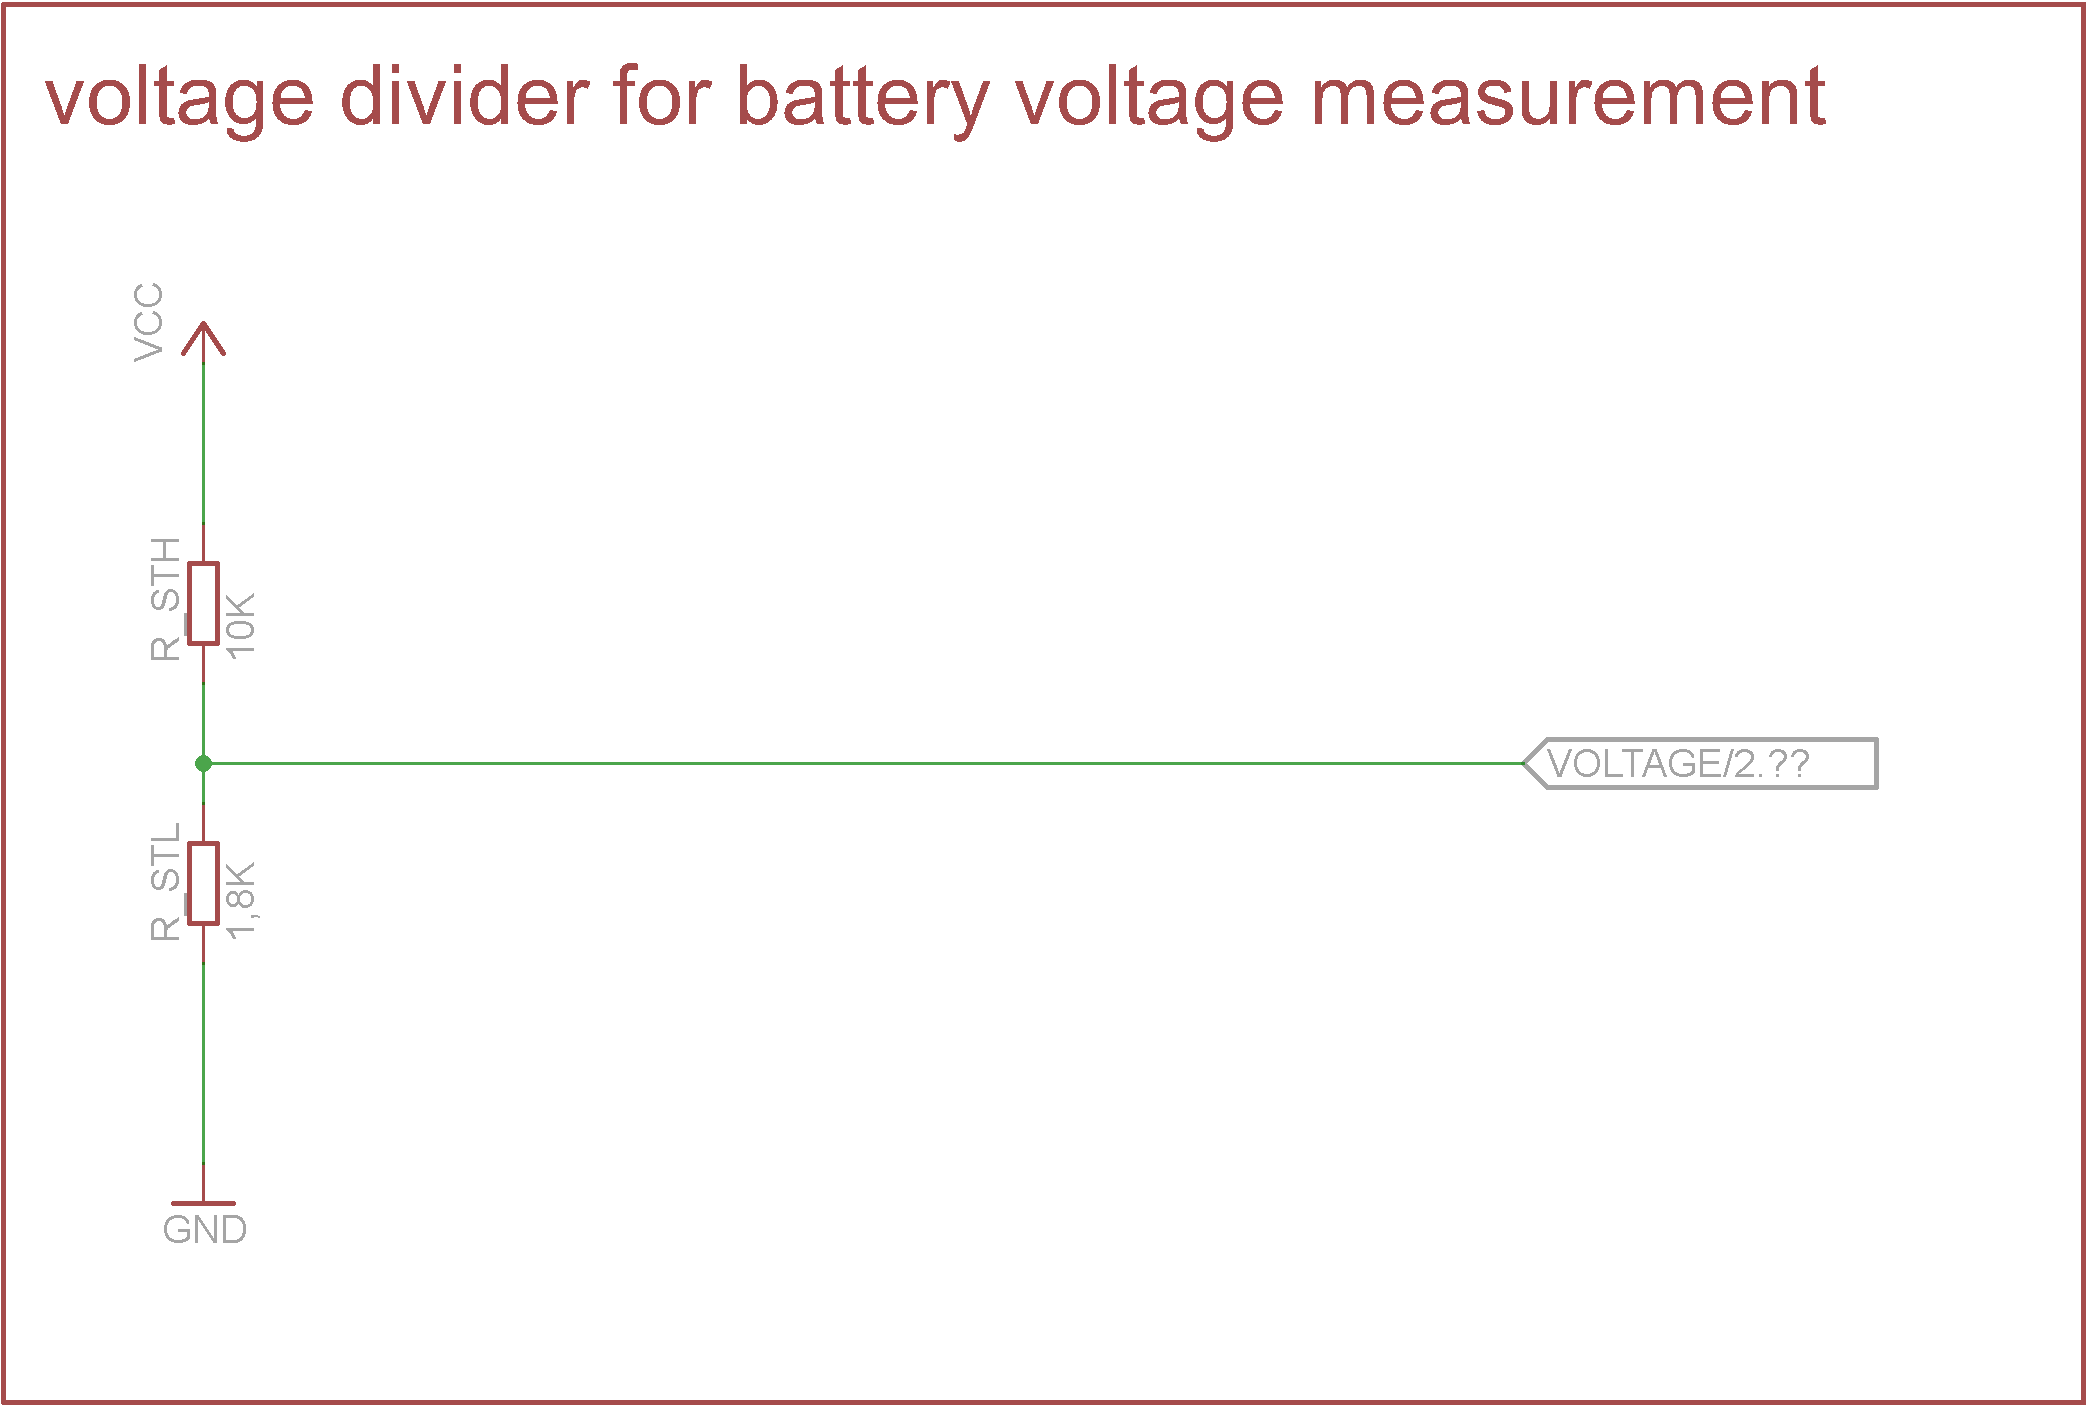
\includegraphics[width=.8\textwidth]{spannungsteiler.png}\\
\caption{Spannungsteiler zur Akkuspannungsmessung}%
\label{fig:Spannungsteiler}
\end{figure}

Da der Innenwiderstand des ADC sehr groß ist (\SI{100}{\mohm}), kann der Spannungsteiler als unbelastet betrachtet werden. Damit ergibt sich das Teilungsverhältnis zu $\frac{R_{STL}}{R_{STH}+R_{STL}}=0,153$.
Die maximal messbare Akkuspannung beträgt dadurch $\frac{\SI{5}{\V}}{0,152}=\SI{32,7}{\V}$. Die Messung des Stroms gestaltet sich wesentlich aufwändiger und wird im Folgenen erläutert.

%TODO
\todo{Maximale Betiebsspannung ermitteln!!}


\subsection{Problem}

Die Messung des Motorstroms ist mit einem Problem behaftet, da der Motor über eine Pulsweitenmodulation angesteuert wird. Der Verlauf des Stoms ist pulsierend, abhängig von
der Frequenz der Pulsweitenmodulation. In \cref{fig:pwm+i_0} zu erkennen ist der Verlauf des PWM Signals (obere Kurve) und des Stoms, welcher nach einer $1-e^t$ Funktion ansteigt.
Ohne weitere Filterung des Signals wäre eine extrem hohe Abtastfequenz des ADC nötig um den genauen Stromfluss zu messen. Da für eine Verbrauchsmessung 
der Mittelwert des Stoms interessant ist, kann dieser mit Hilfe eines Tiefpasses erzeugt werden.


\begin{figure}[H]
\centering
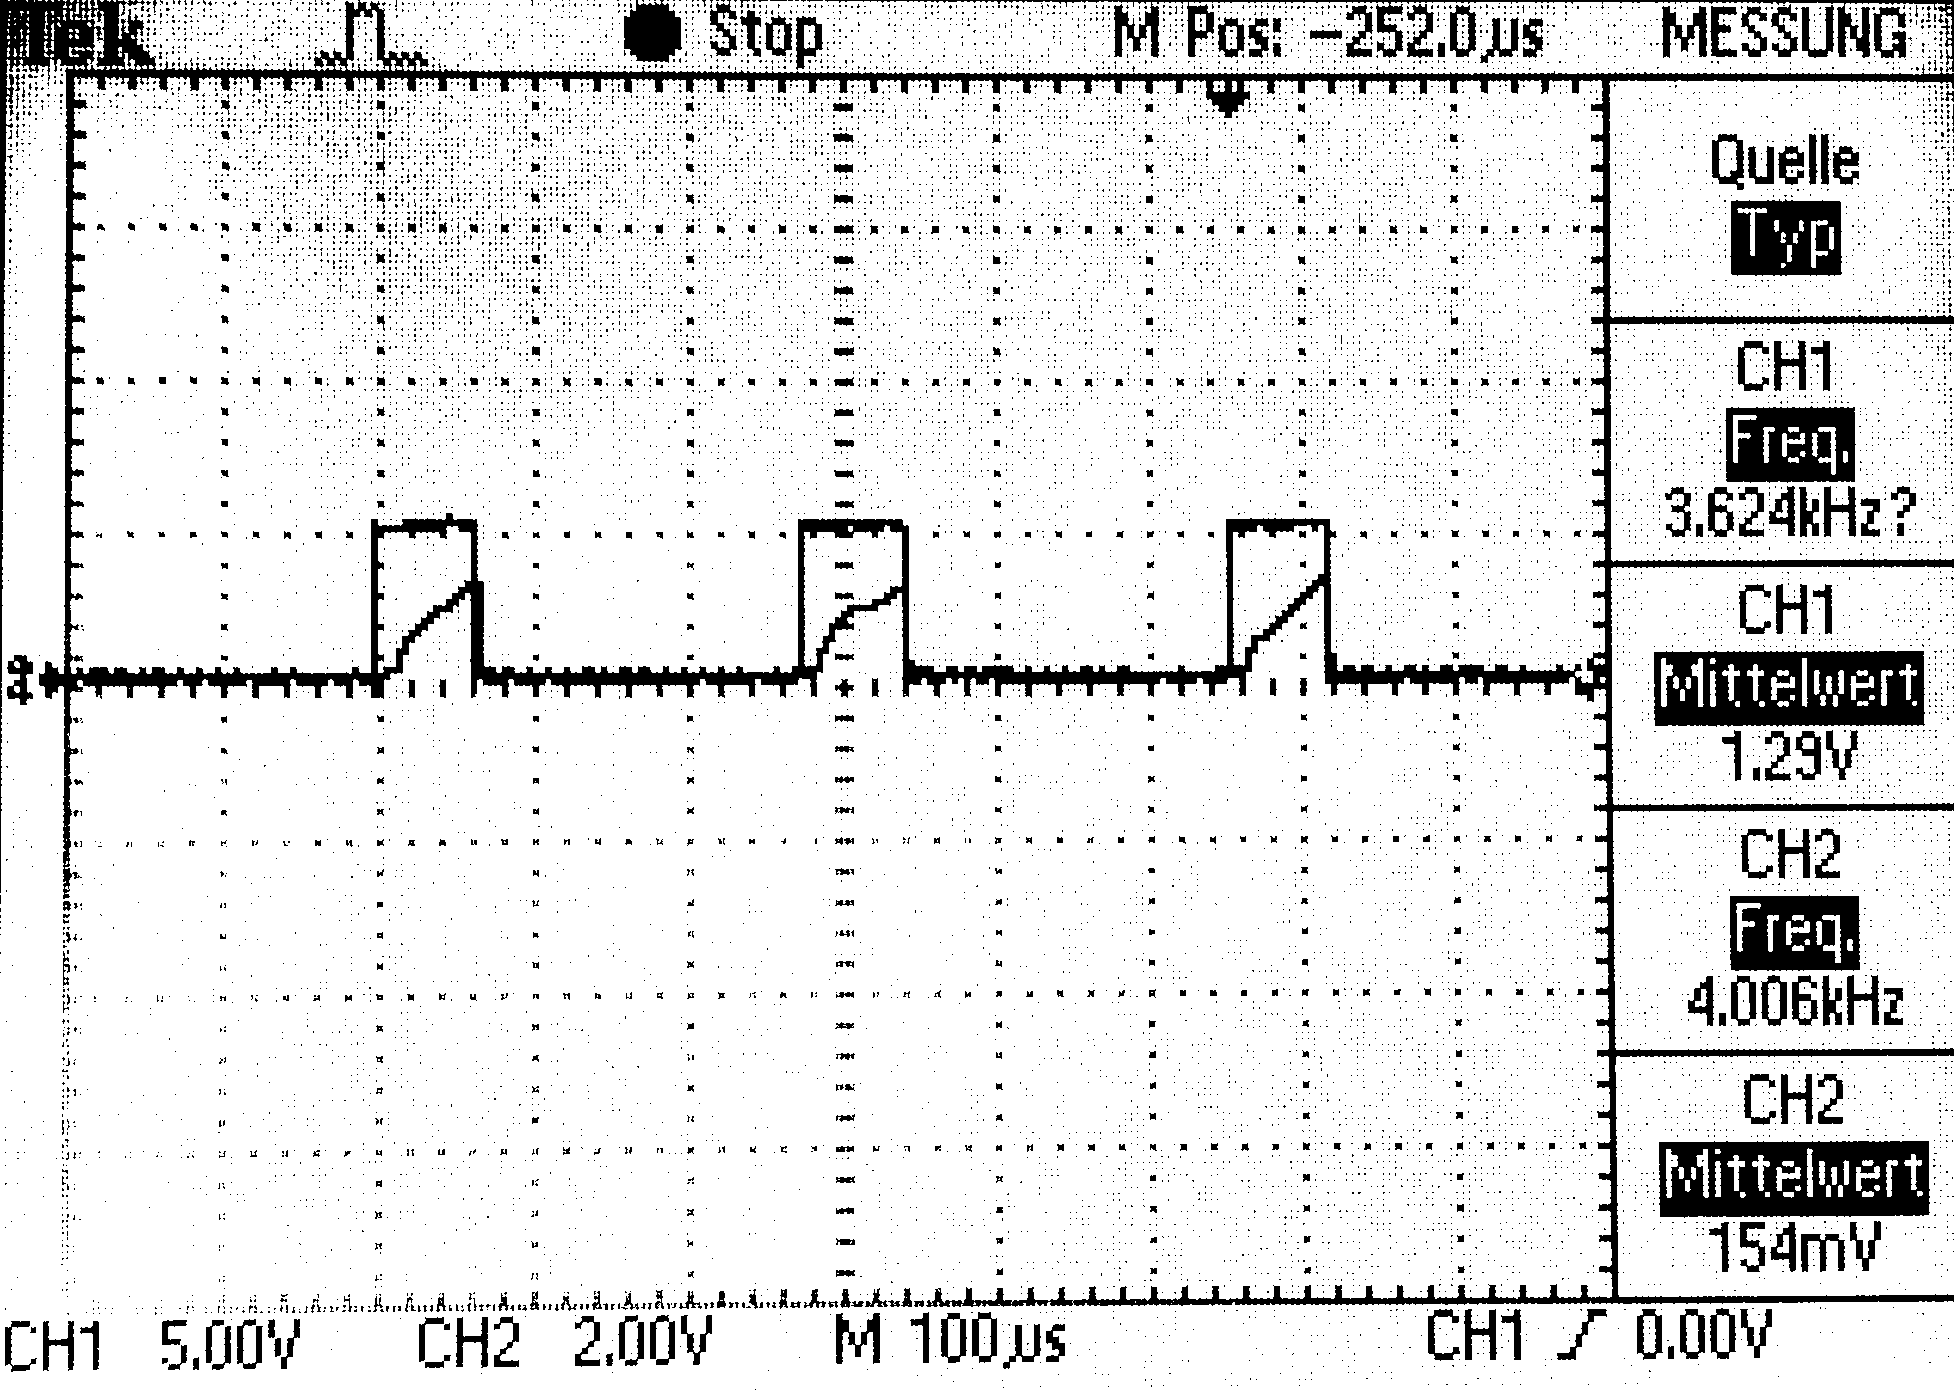
\includegraphics[width=.8\textwidth]{oszi.png}\\
\caption{Spannung am Shunt + PWM}%
\label{fig:pwm+i_0}
\end{figure}

Eine kostengünstige Variante den Strom zu messen ist den Spannungsabfall über einen Shuntwiderstand zu bestimmen. Die Größe des Shuntwiderstandes sollte nur so klein wie nötig gewählt werden.
Ein zu kleiner Shuntwiderstand benötigt einen starken Messverstärker um das Signal auswerten zu können. Die Qualität und Genauigkeit dieses Signals nimmt allerdings mit steigender Verstärkung ab.

Nach kurzer Recherche wurde die Größe des Shuntwiderstands auf R2512(ca \SI{6,35}{\mm} x \SI{3,00}{\mm}) begrenzt. Messshunts in dieser Größe gibt es problemlos bis zu einer Belastbarkeit von 2 Watt. 
Bei einem maximalen Motorstrom von 20A ergibt sich somit ein maximaler Spannungsabfall von \SI{100}{\mV}. Nach dem Ohmschen Gesetz erbib sich so eine Shuntgröße von
$\frac{\SI{0,1}{\V}}{\SI{20}{A}}=\SI{0,005}{\ohm}$. Shuntwiederstände in der Größe sind problemlos zu bekommen.
Da es sich hier um eine Worst Case Rechnung handelt, wird der zusätzliche Widerstand des Shuntwiederstandes und der damit verringerte Strom bewusst ignoriert.

Der Shunt wird direkt unter der H-Brücke des Motortreibers gegen Ground geschaltet. So wird eine Messung gegen Ground durchgeführt. Die so über den Shuntwiederstand gemessene Spannung könnte 
dann über den ADC Eingang des Mikrocontrollers eingelesen werden. Vorher jedoch muss das Signal gefiltert und verstärkt werden.

\subsection{Anforderungen}
Die maximale Auflösung des Mikrocontrollers soll ausgenutzt werden. Der ADC des Mikrocontrollers arbeitet mit einer Auflösung von 10 Bit und einer 
Referenzspannung von 5V. Um die Auflösung des ADC auszunutzen muss das Signal, aufgrund des geringen Spannungsabfalls, verstärkt werden.

Als Anforderung ergibt sich außerdem, dass der maximale Ripple des Endsignals kleiner ist als der Quantisierungsfehler des ADC.
So ist es möglich auf eine zusätzliche digitale Filterung weitgehend zu verzichten.
Die kleinst mögliche zu erfassende Spannung des ADC beträgt $\frac{5}{2^{10}}=4,88mV$.
Diesen Wert sollte der Ripple des Endsignales nicht überschreiten.
Aus einem möglichst kleinem Ripple resultiert eine möglichst hohe Filterordnung bzw. eine niedrige Grenzfrequenz.
Allerdings soll $U_{DC}$ einer Änderung des Mittelwertes, also einer Änderung des Tastverhältnisses, möglichst
schnell folgen. Diese Anforderung widerspricht der Vorherigen, sodass ein Kompromiss gefunden werden muss.

\subsection{Bestimmung des Filtertyps}
Da zum Verstärken des Signals aktive elektronische Elemente notwendig sind, z.B. ein Operationsverstärker, wird an dieser Stelle gleich ein aktiver Filter verwendet. 
Dieser gibt uns die Möglichkeit des Messsignal zu verstärken und gleichzeitig zu
filtern. Da das Signal im optimalen Fall eine Gleichspannung darstellt, müssen die hochfrequenten Anteile des Signales herausgefiltert werden. Dies geschieht 
mit Hilfe eines Tiefpasses. Es gibt im Grunde zwei übliche aktive Tiefpässe, den Tiefpass mit Mehrfachgegenkopplung und den Sallen-Key Filter. Ersterer verwendet
einen invertierenden Verstärker, dieser invertiert das Messsignal. Da der Mikrocontroller jedoch nur mit positiven Spannungen umgehen kann, müsste man hier mit einer 
negativen Referenzspannung arbeiten, was den Schaltungsaufwand unnötig vergrößern würde. Der Sallen-Key Tiefpass benutzt einen nicht invertierenden Verstärker, welcher diesen
Nachteil nicht hat. So dass ab dieser Stelle ein Sallen-Key Tiefpass entworfen wird.

%TODO
\todo{Quellen (verweise auf übliche Filtertypem)}

\subsection{Die Filterschaltung}

Wie im vorherigen Abschnitt diskutiert wird hier ein Sallen-Key Tiefpass entworfen. Zum Entworf der Schaltung [\ref{fig:fschalt}] wurde Eagle genutzt.
\todo{Welcher OPV wird genutzt und warum}

\begin{figure}[H]
\centering
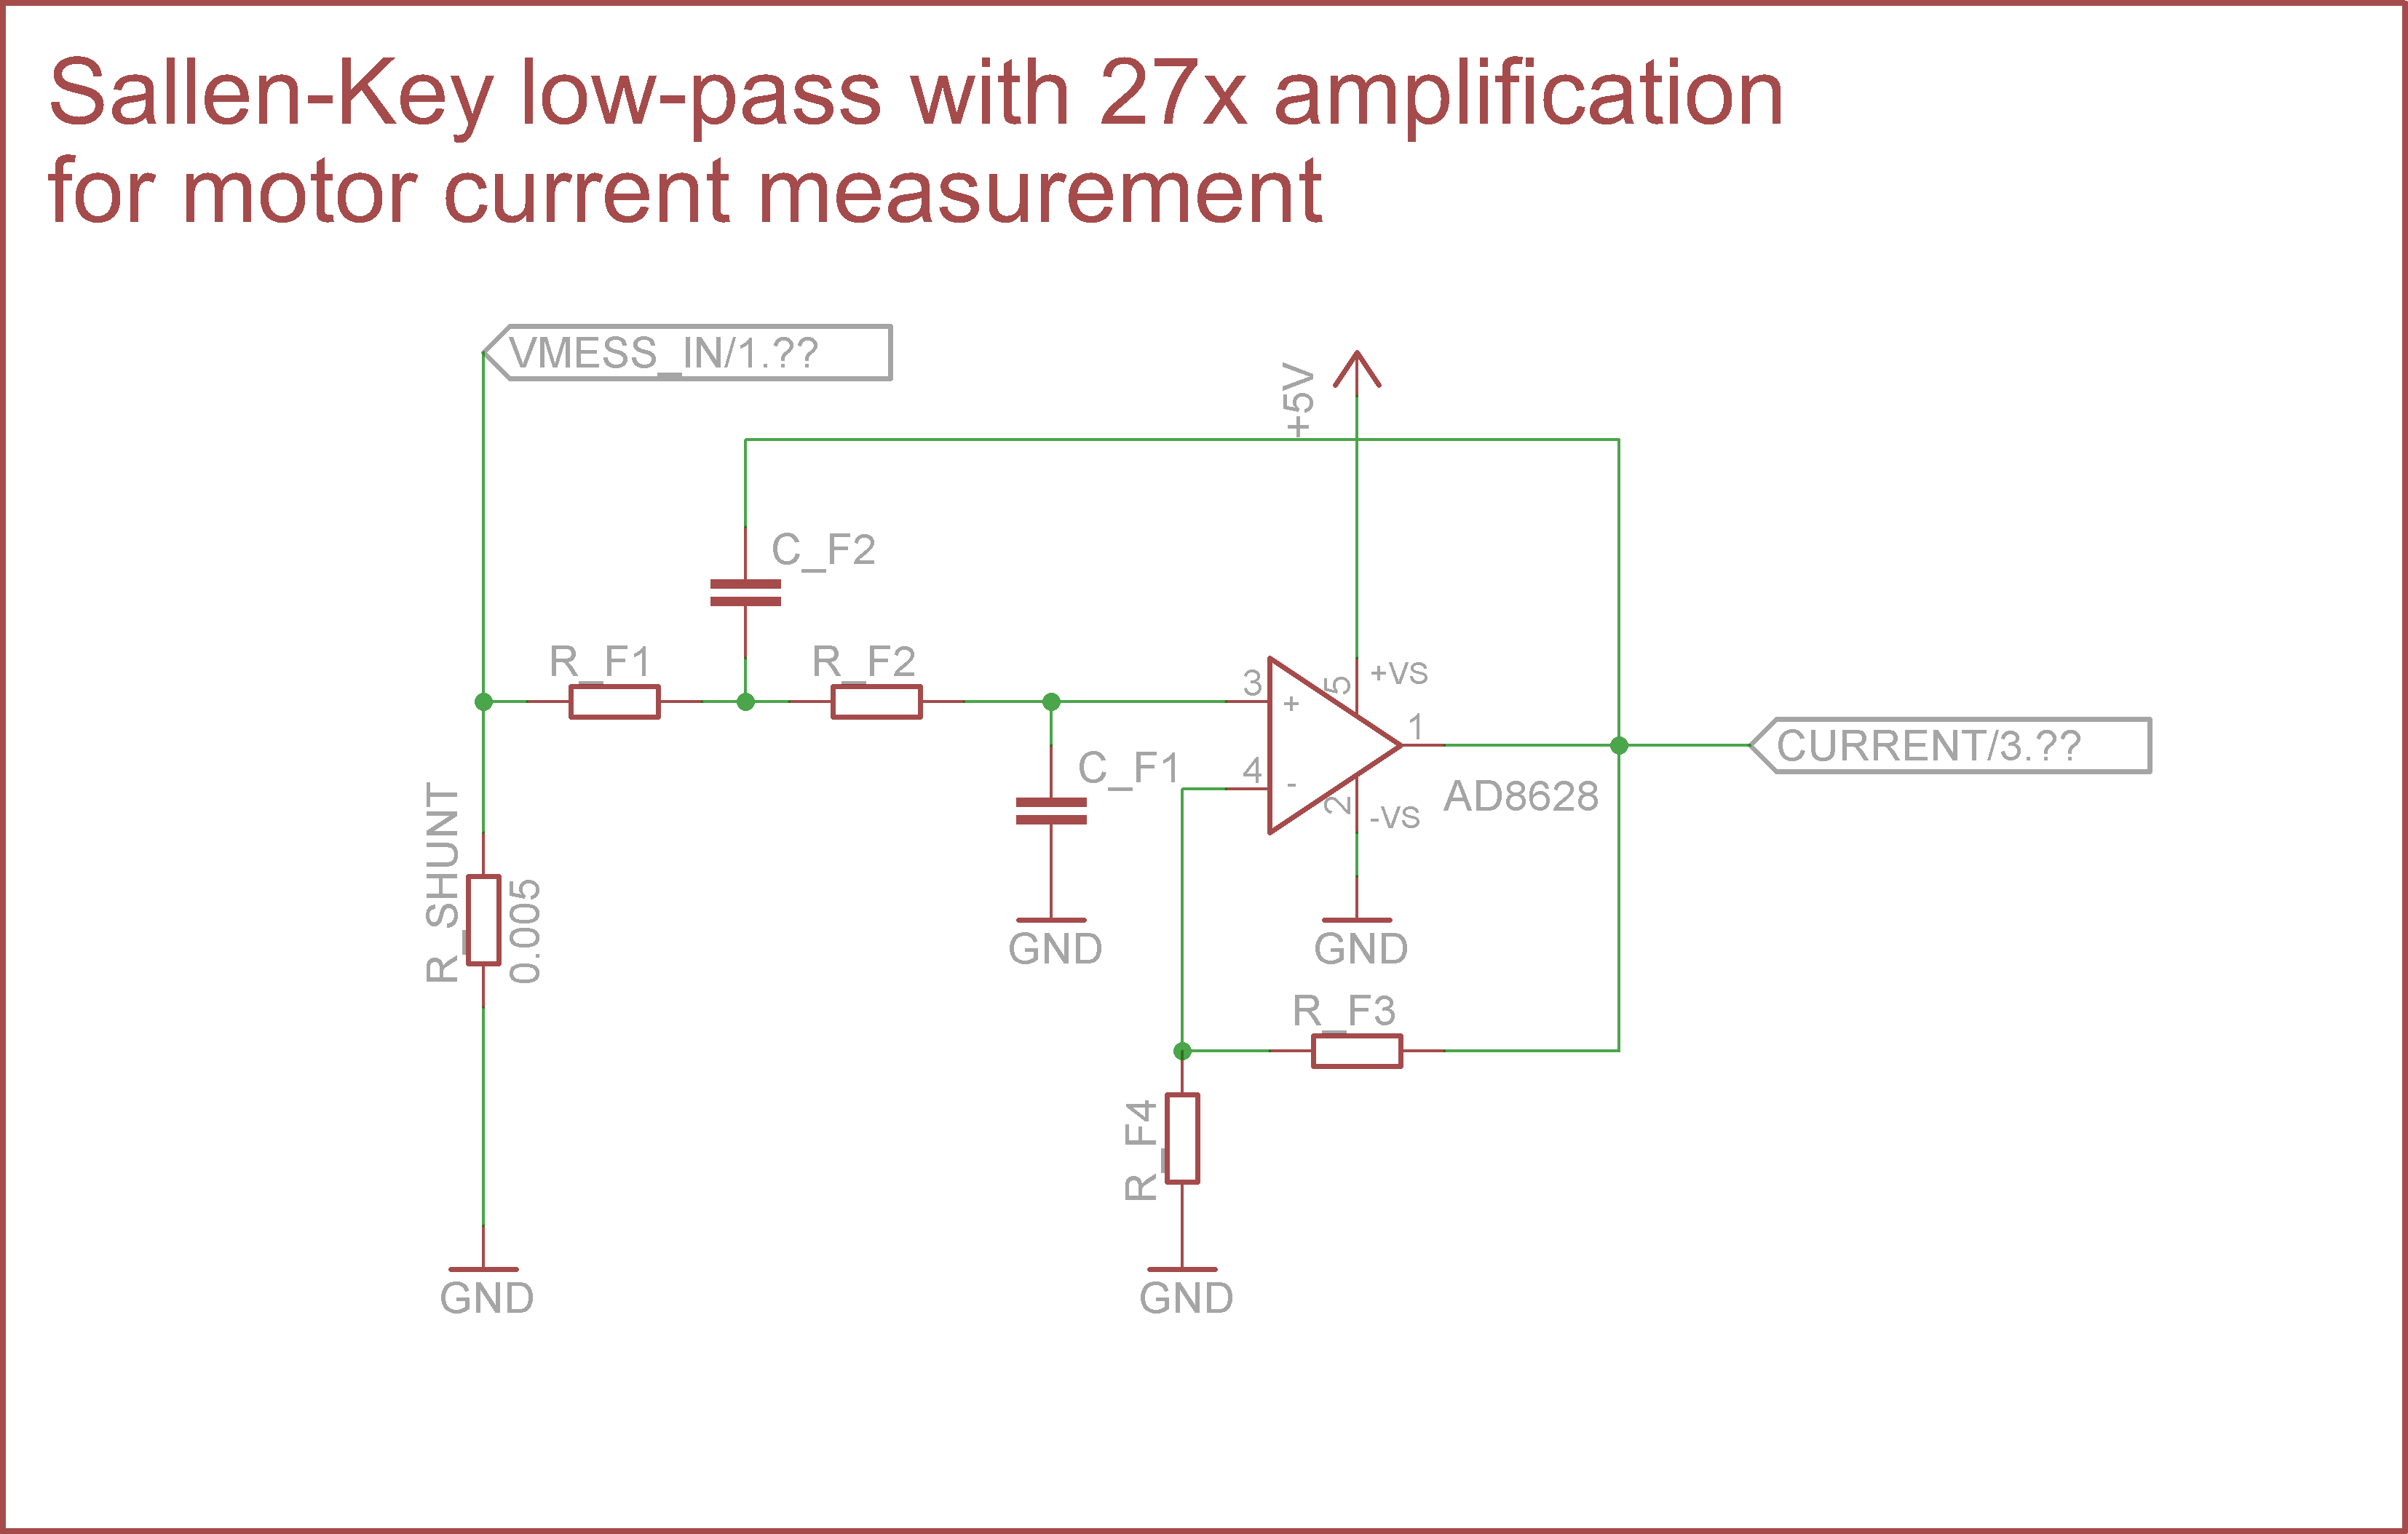
\includegraphics[width=.8\textwidth]{filter_schaltung.png}\\
\caption{Salle-Key Tiefpass mit Shunt}%
\label{fig:fschalt}
\end{figure}



\subsection{Dimensionierung des Verstärkers}

In bisherigen Rechnungen wurde ein maximaler Spannungsabfall von 100mV am Shunt errechnet. Da der Messbereich des ADC voll ausgenutzt werden soll,
ist es nötig das Messsignal zu verstärken. Hierzu wird ein nichtinvertierender Verstärker genutzt. Da der Messbereich des ADC bis 5V reicht, wird hier eine 
50-fache Verstärkung angestrebt.

Die Beschaltung, welche den Verstärkungsfaktor des Sallen-Key Tiefpass festlegt, entspricht der eines nichtinvertierenden Verstärkers:

\begin{align*}
v &= 1 + \frac{R_{F3}}{R_{F4}}\\
50 &= 1 + \frac{R_{F3}}{R_{F4}}\\
49\cdot R_{F4} &= R_{F3}
\end{align*}
\\
Wobei $R_{F4} = 47 k\Omega$ und $R_{F3} = 1 k\Omega$  gewählt werden, was eine Verstärkung von 48 ergibt.

%TODO
\todo{warum werde widerstände so gewählt}

\subsection{Anforderungen an den Filter}

\begin{figure}[H]
\centering
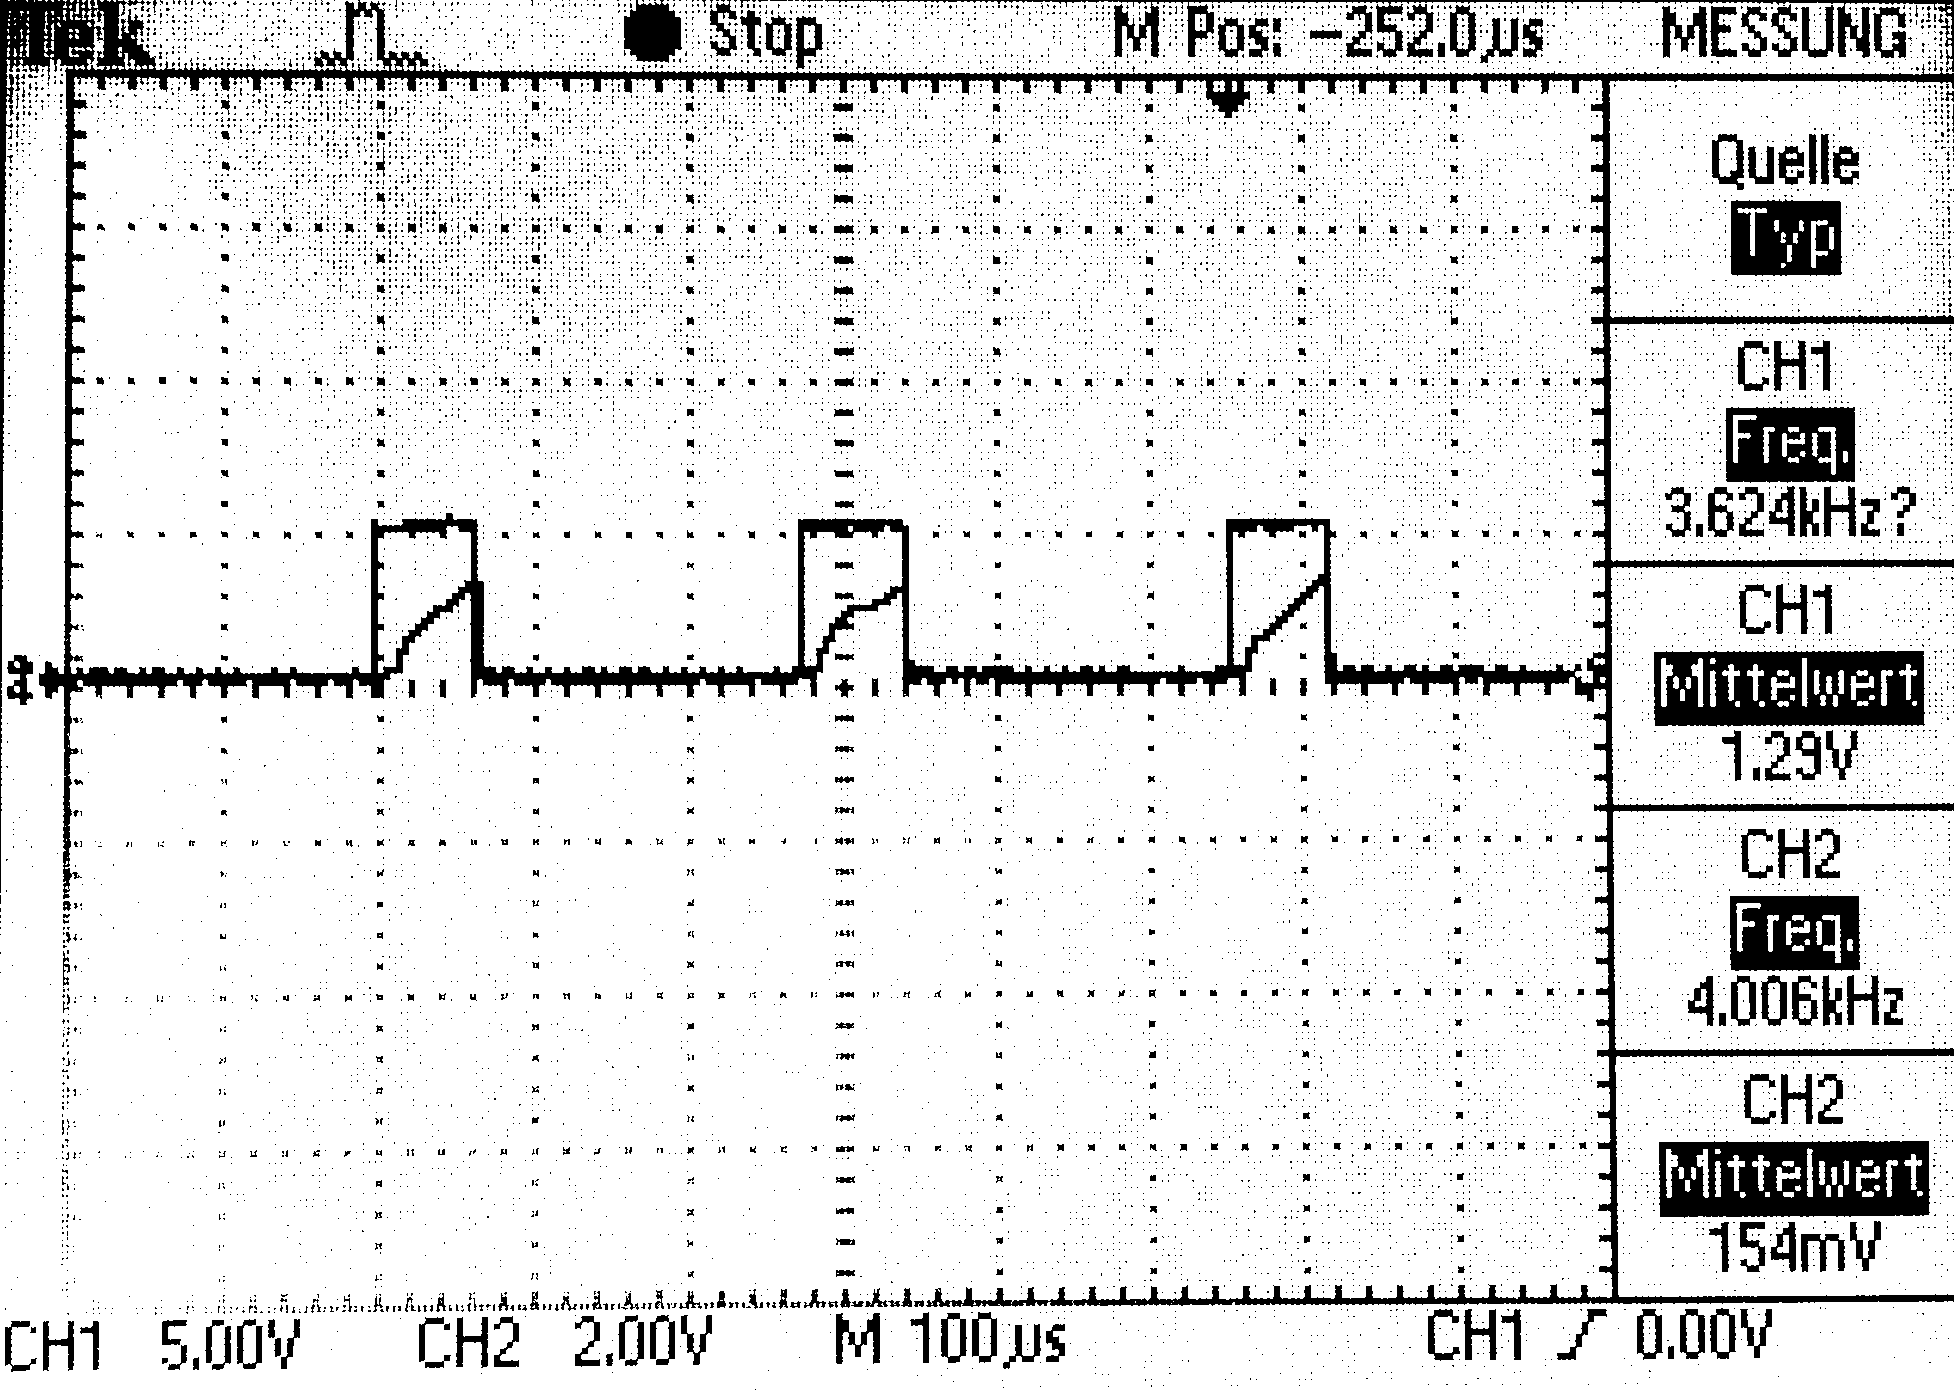
\includegraphics[width=.8\textwidth]{oszi.png}\\
\caption{Spannung am Shunt + PWM}%
\label{fig:pwm+i}
\end{figure}

Da dem Messsignal wie in Abbildung \ref{fig:pwm+i} zu erkennen, die PWM Frequenz zu Grunde liegt, wird sich bei der Dimensionierung des Filters einer Idee nach \cite{Alter2008} bedient, nach der die maximale Amplitude des Ripple der Grundschwingung bei einem
Tastverhältnis von 0,5 entspricht. Die Amplitude der Grundschwingung ergibt sich aus dem ersten Koeffizienten der Fourierreihe einer Rechteckschwingung.
\begin{align}
A_1 = K\cdot \frac{1}{\pi}[\sin(\pi p)-\sin(2\pi(1-\frac{p}{2}))]
\label{eq:ripple}
\end{align}
Wobei $p$ dem Tastverhältnis und $K$ der maximale Amplitude des Ursprungsingals entspricht \cite{Alter2008}. $K$ entspricht den errechneten 100mV multipliziert mit dem Verstärkungsfaktor 48, also 4,8V. Das Tastverhältnis $p$ wird zu 0,5
angenommen. Mit (\ref{eq:ripple}) ergibt sich für die Amplitude der Grundschwingung $ A_1 = K\cdot \frac{2}{\pi} = 3,056V$. $A_1$ soll auf $ < 4,88mV$ gedämpft werden.
Als Sperrfrequenz $\Omega_s $ wird hier die PWM Frequenz angesetzt. Für $H(\omega=2\pi f_{PWM})$ gilt also:

\begin{align}
H(\omega=2\pi f_{PWM}) \le \frac{4,88mV}{3,056V} \mathop{\hat{=}} 20\cdot\log(\frac{4,88mV}{3,056V})= -55,9 dB
\label{eq:daempfung}
\end{align}

Um die Komplexität der Schaltung gering zu halten, wird im Folgenden von den üblichen Konventionen zur Dimensionierung von Filtern abgewichen.
Statt eine fixe Grenzfreqeunz festzulegen und die benötigte Filterordnung zu bestimmen, wird die Filterordnung vorgegeben und die Grenzfrequenz variiert.

\subsection{Filterentwurf}

\subsubsection{Bestimmung des Filtertyps}

Der Filtertyp muss in zweierlei Hinblick bestimmt werden. Einmal im Hinblick auf die Schaltung und seinem Frequenzgang.
Im Groben gibt es zwei mögliche aktive Tiefpassfilterschaltungen, den Sallen-Key Tiefpass mit nicht invertierendem OPV und dem aktiven Tiefpass mit Mehrfachgegenkopplung 
(invertierender OPV). Der aktive Tiefpass mit Mehrfachgegenkopplung benötigt allerdings negative Spannungsniveaus die auf der Treiberplatine nicht zur
Verfügung stehen, deshalb wird an dieser Stelle nur der Sallen-Key Tiefpass betrachtet.
Was den Frequenzgang angeht, gibt es viele Filtercharakteristiken, eine Auswahl an häufig verwendeten Charakteristiken wird hier verglichen.

Der \emph{Butterworth}-Filter besitzt einen maximal flachen Verlauf des Frequenzganges im Durchlassbereich und eine monoton verlaufende Dämpfung im Sperrbereich.
Leider hat der Butterworth-Filter nur eine geringe Flankensteilheit im Sperrbereich (20dB/Dekade pro Ordnung). Ein Butterworth-Filter 1. Ordnung entspricht einen  einfachen RC-Filter.

Der \emph{Tschebyscheff}-Filter hat eine höhere Flankensteilheit als der Butterworth-Filter, allerdings entsteht beim Tschebyscheff-Filter Welligkeit im Durchlassbereich,
welche mit höherer Ordnung zunimmt. Durch die Welligkeit im Duchlassbereich würde ein zusätzlicher Ripple im Signal entstehen, weshalb der Tschebyscheff-Filter nicht
für den geforderten Filter geeignet ist 

Der \emph{Bessel-Filter} hat den Vorteil einer konstanten Gruppenlaufzeit, hat dafür aber eine noch geringere Flankensteilheit als der Butterworth-Filter.
Da eine konstante Gruppenlaufzeit für den geforderten Filter nicht von Vorteil ist, da das Endsignals einer Gleichspannung entsprechen sollte, ist der Butterworth-Filter
die bessere Wahl.


\begin{figure}[H]
\centering
\begin{tikzpicture}
	\draw[->,thick] (0,0) -- (7.5,0) node[right] {$f[\text{Hz}]$};
	\draw[->,thick] (0,0) -- (0,3.3) node[above] {$a[\text{dB}]$};
	\draw (0,2.5)node[left] {$a_{\text{min}}$} (-0.1,2.5)--(2.9,2.5);
	\draw (0,1)node[left] {$a_{\text{max}}$};
	\def \bsp{(0,1)--(1,1)--(1,2.4)--(1,2.4)--(0,2.4)}
	\draw (-0.1,1)--(1,1)--(1,2.4) (1,0)node[below] {$f_g$};
	\pattern[pattern=north east lines] \bsp;
	\draw[dashed] (1,1) -- (1,-0.1);
	\def \bsd{(3,0) -- (3,2.5) -- (7,2.5) -- (7,0)}
	\pattern[pattern=north east lines] \bsd;
	\draw (3,0)node[below] {$f_s$} -- (3,2.5) -- (7,2.5);

\end{tikzpicture}
\caption{Tiefpass Toleranzfeld}%
\label{fig:analog}
\end{figure}



Für unsere Schaltung wird ein Sallen Key Tiefpass 2. Ordnung nach Butterworth entwurfen. Die PWM-Frequenz $f_{PWM}$ beträt 3,9kHz.
%TODO
\todo{PWM Frequenz muss noch festgelegt werden, hier sonst erste erwähnung....}
Die Sperrfrequenz entspreicht der PWM Frequenz, also der Frequenz unserer Grundschwingung. $\Omega$ entspricht der mit der Grenzfreqeunz 
normierten Frequenz $\Omega=\frac{f}{f_g}$. Nach (\ref{eq:daempfung}) ergibt sich für Abbildung \ref{fig:analog}
$f_s=f_{PWM}=3,9 kHz$, $a_{min}=55,9 dB$ und $a_{max}$ wird auf 3dB festgelegt.






\subsubsection{Bestimmung der Grenzfreqeunz}
\begin{align}
n \ge \frac{\log{\sqrt{\frac{e^{2a_{min}}-1}{e^{2a_{max}}-1}}}}{\log{\Omega_s}}
\label{eq:butterworth}
\end{align}
Die Filterordnung nach Butterworth wird nach (\ref{eq:butterworth}) bestimmt. Umgestellt nach $\Omega_s$ ergibt sich:

\begin{align}
\Omega_s \le  \left(\frac{e^{2a_{min}}-1}{e^{2a_{max}}-1}\right)^{\frac{1}{2n}}
\end{align}



Für die Berechnung der Sperrfrequenz $\Omega_s$ müssen  $a_{min}$ und $a_{max}$ in Neper umgrechnet werden. Wobei:
\begin{align*}
1 \text{dB} =  \frac{\ln{10}}{20}\text{Np} = 0,115129255 \text{Np}   
\end{align*}

Damit ergibt sich für $a_{min}=55,9 dB\cdot \frac{\ln{10}}{20}=6,45Np$ und für  $a_{max}=3 dB\cdot \frac{\ln{10}}{20}=0,345Np$. Die Filterordnung wird auf 2 festgelegt.
\begin{align}
\Omega_s \le  \left(\frac{e^{2\cdot6,45N }-1}{e^{2\cdot 0,345Np}-1}\right)^{\frac{1}{2n}}  = 35,8
\end{align}

Die Grenzfreqeunz $f_g$ ergibt sich jetzt aus:

\begin{align}
\frac{f_s}{\Omega_s} \le \frac{3,9kHz}{35,8} = 108,9Hz
\end{align}

\subsubsection{Filterentwurf}
Im voherigen Abschnitt wurde berechnet, dass die Grenzfreqeunz des Filters kleiner als 108,9Hz sein muss.
Im Folgenden wird nun ein Sallen-Key Filter 2. Ordnung mit einer Grenzfrequenz von 100Hz entworfen.
Die genaue Wahl der Grenzfreqeunz ist hier nicht relevant da die realen Bauteile nicht in  allen Größen 
verfügbar sind und daher am Schluss variiert werden müssen, wodurch sich die Grenzfrequen des Filters leicht ändert.


\subsubsection{Finaler Entwurf}



Betrachten wir das Polstellen-Nullstellendiagramm eines Butterworth Filters 2. Ordnung, wie in [\cref{fig:filter_polnul}]


\begin{figure}[H]
\centering
\begin{tikzpicture}
	\draw[->,thick] (-3,0) -- (3,0) node[right] {$\text{Re}$};
	\draw[->,thick] (0,-3) -- (0,3) node[above] {$\text{Im}$};
	\draw[dashed,red,very thin] (-3,2) -- (3,2);
	\draw[dashed,red,very thin] (-3,-2) -- (3,-2);
	\draw[dashed,red,very thin] (2,-3) -- (2,3);
	\draw[dashed,red,very thin] (-2,-3) -- (-2,3);
	\draw[dashed,blue,very thin] (0,0) circle (2);
	\coordinate (x) at (225:2); 
	\coordinate (y) at (135:2);
	\draw[very thin] (0,0) -- (y);
	\draw[red,thick] (x) -- +(0.1,0.1)  (x) -- +(-0.1,-0.1) (x) -- +(0.1,-0.1) (x) -- +(-0.1,0.1);
	\draw[red,thick] (y) -- +(0.1,0.1)  (y) -- +(-0.1,-0.1) (y) -- +(0.1,-0.1) (y) -- +(-0.1,0.1);
	\draw (2,0)node[below] {$1$};
	\draw (-2,0)node[below] {$-1$};
	\draw (0,2)node[left] {$1$};
	\draw (0,-2)node[left] {$-1$};
	\draw (0,-2)node[left] {$-1$};
	\draw (0,0) (135:1cm) arc (135:180:1cm);
	\draw (-0.6,0.3)node {$\delta$};
\end{tikzpicture}
\caption{Polstellen-Nullstellendiagramm, Butterworth 2. Ordnung}
\label{fig:filter_polnul}
\end{figure}



Charakteristisch für den Butterworthfilter ist, dass sich die Polstellen auf einer Kreisbahn befinden. Auf die Grenzfreqeunz normiert hat dieser beim Butterworthfilter den Radius
eins. Bei einem Butterworth 2. Ordnung befinden sie sich genau bei $\delta=45^\circ$. Das Interessante am Polstellen-Nullstellendiagramm ist, dass sich Polfrequenz $\Omega_P$ und 
Polgüte $Q_P$ einfach ablesen lassen. Die Polfrequenz $\Omega_P$ ist der Betrag der normierten Polstelle, welcher beim Butterworth-Filter immer eins ist.
Die Polgüte ist abhängig von $\delta$ und ergibt sich zu: $Q_P=\frac{1}{2\cos{\delta}}$. Für unseren Butterworthfilter ergeben sich also $Q_P=0,707$ und $\Omega_P=1$

%TODO
\todo{Variablennamen auf Schaltplan anpassen}

Betrachten wir die Übertragungsfunktion eines Sallen-Key Tiefpasses 2. Ordnung:

\begin{align*}
A(P)&=\frac{A_0}{1+\omega_g (R_2 C_2 + R_1 C_2 + R_1 C_2(1-A_0))P + \omega_g^2R_1 R_2 C_1C_2P^2}
\end{align*}

mit
\begin{align*}
A_0=1+\frac{R_6}{R_5}
\end{align*}


Die Bauteilwerte erhält man durch einen Koeffizientenvergleich mit der entnormierten
Übertragungsfunktion ($P=\frac{s}{\omega}$) eines Tiefpasses zweiter Ordnung:

\begin{align*}
A(P)&=\frac{A_0}{1+\frac{1}{\omega_g\Omega_PQ_P}s+\frac{1}{\omega_g^2\Omega_P^2}s^2}
\end{align*}

Die Auflösung des Vergleiches ist mit vielen mathematischen Umformungen verbunden, deswegen wird hier auf eine
externe Quelle verwiesen \cite[S. 102]{Krucker2000}.
Nach dem Koeffizientenvergleich ergibt sich

\begin{align*}
C_1&<\frac{C_2\cdot(1+4Q^2_P(A_0-1))}{4Q^2_P}\\
R_1&=\frac{1}{2\omega_g\Omega_PQ_P} \cdot \frac{C_2\pm\sqrt{C_2^2-4Q^2_PC_2(C_1+C2(1-A_0))}}{C_2(C_1-C_2(1-A_0))}   \\
R_2&=\frac{1}{2\omega_g\Omega_PQ_P} \cdot \frac{C_2\pm\sqrt{C_2^2-4Q^2_PC_2(C_1+C2(1-A_0))}}{C_1C_2}  \\
Q_p&=\frac{\sqrt{R_1R_2C_1C_2}}{C1(R_1+R_2)+R_1C_2(1-A_0)}\\
\Omega_p&=\frac{1}{\omega_g\sqrt{R_1R_2C_1C_2}}
\end{align*}

Dabei sind immer nur die positiven, reellen Lösungen zu verwenden.


\subsubsection{Bestimmung der Bauteilwerte}

Um die Übersicht zu wahren wird die Berechnung der Bauteilwerte hier nicht aufgeführt. Zur Erinnerung,
die gegebenen Werte sind $Q_P=0,707$, $\Omega_P=1$, $A_0=48$ und $\omega_g = 2 \cdot \pi 100Hz$.
$A_0$ ist die Gleichspannungsverstärkung, sie beschreibt den gewünschten Verstärkungsfaktor der bereits in einem voherigen
Abschnitt mit 48 bestimmt wurde. Die Berechnungen wurden mit Hilfe eines Python-Scriptes ausgeführt, dabei wurden verschiedene
Konfigurationen durchgerechnet. Hautpsächlich wurde dabei darauf geachtet, dass sich der Filter mit den vor Ort vorhandennen SMD-Bauteilen
aufbauen lässt.

In den Berechnungen fiel auf, dass bei steigender Größe der Kondensatoren die Größe der Widerstände sinkt. Da Widerstände auch in großen Größen vorhanden waren,
wurde für den frei wählbaren $C_2$ ein kleiner Wert von 82nF gewählt.

\begin{align*}
C_1&<\frac{C_2\cdot(1+4\cdot0.707^2_P(48-1))}{4\cdot0.707^2}\\
C_1&<3.90\mu F
\end{align*}

$C_1$ soll nur kleiner sein als 3.90\textmu F und wird ebenfalls auf 82nF gesetzt.

\begin{align*}
R_1&=\frac{1}{2\cdot100Hz\cdot0,707} \cdot \frac{82nF\pm\sqrt{82nF^2-4\cdot0.707^2\cdot82nF(82nF+82nF(1-48))}}{82nF(82nF-82nF(1-48))}\\
R_1&=[-3176\Omega,2579\Omega]
\end{align*}


\begin{align*}
R_2&=\frac{1}{2\cdot100Hz\cdot0,707} \cdot \frac{82nF\pm\sqrt{82nF^2-4\cdot0.707^2\cdot82nF(82nF+82nF(1-48))}}{82nF^2}\\
R_2&=[146079\Omega,-118626\Omega]
\end{align*}

Da nur positive Werte genutzt werden, ergeben sich die Bauteilwerte nun zu:
\begin{align*}
C_1&=82nF\\
C_2&=82nF\\
R_1&=2579\Omega\\
R_2&=146079\Omega
\end{align*}

In der folgenden Abbildung ist das Ergebnis der Simulation zu sehen. An der Abbildung leider nicht gut zu erkennen,
liegt der -3dB Punkt genau bei 100Hz. Die Frequenzachse des Diagrammes geht genau bis 3,9kHz. 
Es ist eine Verstärkung von 48 des Ursprungssignals gewünscht. Diese Verstärkung wird mit 33,6 dB bei 10Hz, erreicht.
\begin{align*}
20\cdot\log{48}=-33,6dB
\end{align*}

Bei 3,9kHz erreicht der Filter eine Dämpfung von -30,1dB. Zusammen mit der Verstärkung von 33,6dB unseres Eingangssignals 
wird das bereits verstärkte Signal also um 63,7 dB gedämpft. Gefordert waren hier 55,9dB, so dass der Filter den gerforderten Wert übersteigt, was an der niedrigeren Grenzfreqeunz von 100Hz statt 108,9Hz liegt.

%%Verstärkung: 33,6dB gewünscht:
%%20*log(1/48)=-33,6

%%dämpfung bei 3,9Khz = 30,7dB
%% 33,6+30,1 =63,7 gewüncht: 55,9
%% Grenzfreqeunz = 100Hz (-3db)
\begin{figure}[H]
\centering
\begin{gnuplot}[terminal=pdf]
  set nokey 
  set xrange [10:3900]
  set xlabel 'Frequenz in [Hz]'
  set ylabel 'Verstärkung in [dB]'
  set logscale x 10
  plot 'Simulation/Filter_original_frequenzgang.csv' with line
\end{gnuplot}
\caption{Frequenzgang des berechneten Filters}
\label{plott:filter_freq}
\end{figure}

Leider kann ein solcher Filter nur mit erheblichen Aufwändungen gebaut werden, da es keine fertigen Widerstände in den Größen $2579\Omega\\$ und $146079\Omega$ gibt. Da jedoch alle Widerstände der E12 Reihe vor Ort vorhanden sind, werden die realen Werte wie folgt gewählt: $R_1=2,7k\Omega\\ R_2=150k\Omega$, da sie den nächsten Größen in der E12 Reihe entsprechen.


In der folgenden Abbildung ist die Simulation des Filters mit den realen Bauteilwerten(grün) im Vergleich zum idealen Filter(rot) zu sehen.
Die Grenzfrequenz des Filters (-3dB) liegt diesmal mit 104Hz etwas über den ursprünglichen 100Hz. Da wir die Werte von $R_5$ und $R_6$ nicht verändert haben, liegt die Verstärkung bei 10Hz immer noch bei exakt 33,6dB. Bei 3,9 kHz, im Diagramm gut zu erkennen wird trotz der höheren Grenzfrequenz eine höhere Dämpfung als vorher erreicht. Diese liegt bei 33,7dB. Daran kann man erkennen, dass es sich nicht mehr um einen idealen Butterworthfilter handelt. 

\todo{Butterworthfilter identische Schreibweise}
%%Verstärkung: 33,6dB gewünscht:
%%20*log(1/48)=-33,6

%%dämpfung bei 3,9Khz = 30,7dB
%% 33,6+30,7 =64,3 gewüncht: 55,9
%% Grenzfreqeunz = 104Hz (-3db)
\begin{figure}[H]
\centering
\begin{gnuplot}[terminal=pdf]
  set nokey 
  set xrange [10:3900]
  set xlabel 'Frequenz in [Hz]'
  set ylabel 'Verstärkung in [dB]'
  set logscale x 10
  
  plot 'Simulation/Filter_original_frequenzgang.csv' with line linecolor rgb "red", 'Simulation/Filter_real_frequenzgang.csv' with line linecolor rgb "green"
\end{gnuplot}
\caption{Frequenzgang des berechneten Filters mit finalen Bauteilwerten}
\label{plott:filter_freq_real}
\end{figure}


Im der folgenden Abbildung [\ref{plott:filter_sprungantwort}] ist die Antwort des Filters auf ein Rechtecksignal mit 3,9kHz, einem Tastverhältnisvon 0,5 und einer Amplitude von 50mV zu sehen. Das Überschwingen im Bereich von 7ms ist charakteristisch für den Butterworthfiter und wirkt sich negativ auf die Messung des Stromes aus. Allerdings werden solch große Sprünge in der Praxis nicht auftreten, da der Strom duch die große Induktivität des Motors nur langsam ansteigt.
\begin{figure}[H]
\centering
\begin{gnuplot}[terminal=pdf]
  set nokey 
  set yrange [0:3]
  set xlabel 'Zeit in [s]'
  set ylabel 'Spannung in [V]'
  plot 'Simulation/Filter_real_time.csv' with line
\end{gnuplot}
\caption{Sprungantwort des Filters}
\label{plott:filter_sprungantwort}
\end{figure}


Die in Abbildung [\ref{plott:ripple}] gut zu erkennende Restwelligkeit (Ripple) beträgt 3,36mV,und liegt damit deutlich unter den gerforderten 4,88mV. Als Eingangssignal dient hier ein Rechtecksignal mit 3,9kHz und einem Tastverhältnis von 0,5, die Amplitude liegt bei 50mV. Die Tatsache dass das Signal 240mV über den rechnerischen 2,40V  ($0.5V \cdot 48 $) liegt, rührt daher, dass LT-Spice die Steig- und Fallzeiten in den low-Bereich des Rechtecksignals legt, woduruch der Mittelwert des Signals bei 2,64V liegt.
 
%% Ripple: 0,003358
%% zu hoher Spannungswert durch Steig und Fallzeiten im low bereich des Rechtecksignals
\begin{figure}[H]
\centering
\begin{gnuplot}[terminal=pdf]
  set nokey 
  set xrange [0.03:0.04]
  set yrange [2.62:2.66]
  set xlabel 'Zeit in [s]'
  set ylabel 'Spannung in [V]'
  plot 'Simulation/Filter_real_time.csv' with line
\end{gnuplot}
\caption{Restwelligkeit des Filters}
\label{plott:imu_servo}
\end{figure}

Da der berechnete Filter den Anforderungen bestens genügt, wird dieser in die Schaltung übernommen.

\section{Beleuchtung}
Die einfachste Möglichkeit eine Beleuchtung am Auto zu realisieren sind Leuchtdioden, welche in allen erdenklichen Farben zu bekommen sind. Weiter Vorteile
sind ihre Energieeffizienz und günstige Preise. LEDs stellen zudem keine großen Anforderugen an die Energieversorgung.

Das Hauptproblem bei der Integration von vielen LEDs ist die Verkabelung. Eine große Erleichterung bei der Integration sind 
LED-Streifen. Diese LED-Streifen gibt es in vielen Ausführungen. Für diese Arbeit interessant sind allerdings nur jene Vertreter, welche die Ansteuerung
jeder einzelnen LED zulassen. Die LED-Streifen mit Controllern von ``Worldsemi'' sind hierbei die prominentesten Vertreter. Zu erwähnen wären hierbei die Modelle
WS2801, WS2811 und WS2812. Der WS2812 ist dabei nahezu identisch mit dem WS2811 mit dem Unterschied, dass der WS2812 bereits in eine RGB-LED integriert ist.
Im Unterschied zum WS2801 werden die beiden duche eine einzige Signalleitung mit fixem Takt angesteuert, so dass hier eine seperate Taktleitung entfällt.

Der Nachteil an dieser Methode ist, dass das Timing genau eingehalten werden muss um die Daten korrekt zu übertragen. Wie in Abbildung \ref{fig:led_cascade}werden die LEDs kaskadiert. Die Daten werden dann durch die LEDs geschoben.

\begin{figure}[H]
\centering
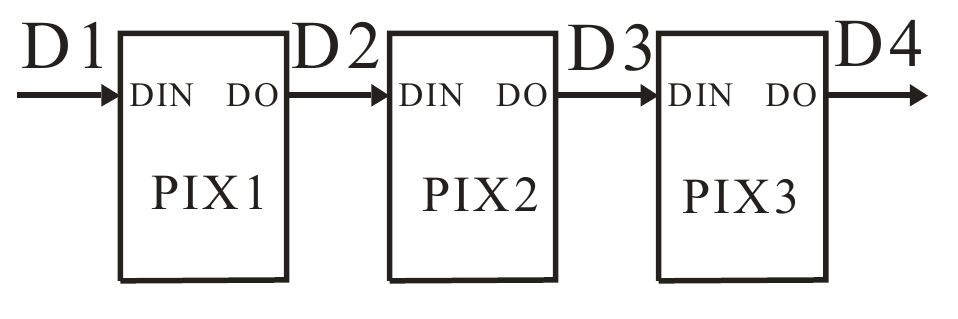
\includegraphics[width=.8\textwidth]{led_cascade.png}\\
\caption{Kaskadierung der LEDs \cite{ds-WS2812}}%
\label{fig:led_cascade}
\end{figure}

Um die Beleuchtung am Auto zu realisieren, werden LEDs mit WS2812 genutzt. Da die LEDs an einem beliebigen
Eingang des AVR-Microcontrollers angeschlossen werden können, wird der LED-Streifen an Pin PA5 angeschlossen. Da das Timing 
exakt eingehalten werden muss, ist die Software zur Ansteuerung in Assember geschrieben.

Die LEDs werden wie folgt angesteuert:\\
Jede LED wird mit einem 24Bit Datenwort angesprochen, welches die Helligkeitsstufen für jede der drei Grundfarben enthält. 
Die Reihenfolge der Daten ist dabei grün, rot und dann blau. Das höchstwertige Bit wird zuerst übertragen.
Die Daten werden ohne Pause gesendet, bis alle LEDs im Strang die nötigen Daten erhalten haben. Nach jeder Übertragung muss eine Pause von mindestens 50\textmu s eingehalten
werden, damit die LEDs die Daten übernehmen. Die einzenen Bits der Übertragung sind dabei folgendermaßen codiert:

\begin{figure}[H]
\centering
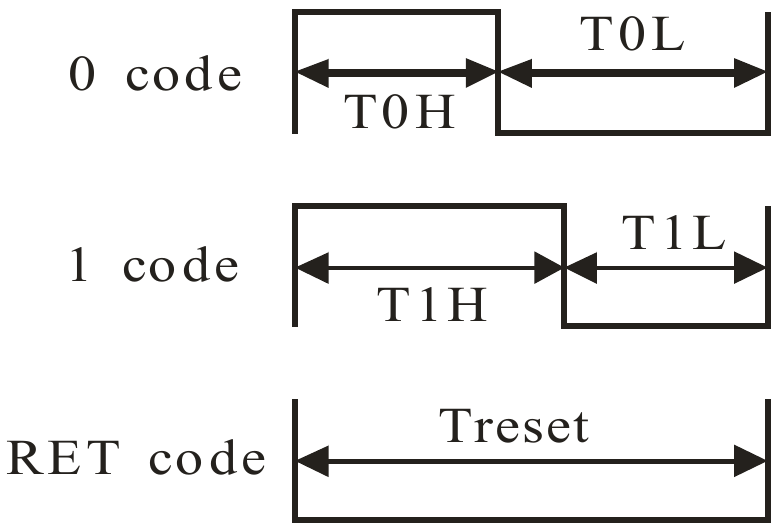
\includegraphics[width=.5\textwidth]{led_timing.png}\\
\caption{Codierung des LED Signals \cite{ds-WS2812}}%
\label{fig:led_timing}
\end{figure}

Die genauen Signallängen können \cref{tab:led_timing} entnommen werden.

\begin{table}[H]
  \centering
  \begin{tabularx}{\textwidth}{|r|X|r|r|}
    \hline
    Abschnitt & Beschreibung & Dauer & Abweichung \\ \hline
    T0H & 0 Code, high Zeit & $0.35\mu s$ & \textpm 150ns\\ \hline
    T1H & 1 Code, high Zeit & $0.7\mu s$ & \textpm 150ns\\ \hline
    T0L & 0 Code, low Zeit & $0.8\mu s$ & \textpm 150ns\\ \hline
    T1L & 0 Code, low Zeit & $0.6\mu s$ & \textpm 150ns\\ \hline
    RES & Reset Code, low Zeit & über $50\mu s$ & \\ \hline
  \end{tabularx}
  \caption{Signallängen}%
  \label{tab:led_timing}
\end{table}




\section{Distanzsensoren}

 
\subsection{Messprinzip}
Die ausgewählen Sensoren der Sharp GP2D Reihe basieren auf einer optischen Abstandsmessung, genauer der optischen Abstandsmessung durch Triangulation.
Bei der optische Abstandsmessung durch Triangulation projiziert ein Projektor einen Lichtpunkt auf das Messobjekt [\ref{fig:lasertriangulation}]. Ein optischer
Sensor misst dann den Winkel des vom Messobjekt reflektierten Lichts. Durch Triangulation kann dann durch den fest definierten Abstand des optischen
Sensors von der Lichtquelle die Entfernung zum Objekt berechnet werden. \cite{Hugenschmidt2007}. In \cref{fig:lasertriangulation} ist
dieses Prinzip veranschaulicht.
\begin{figure}[H]
\centering
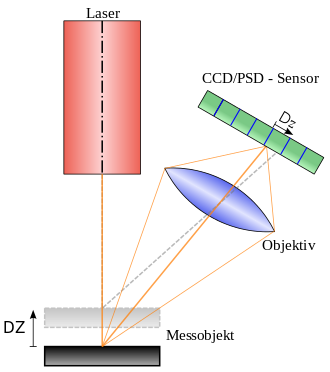
\includegraphics[width=.5\textwidth]{lasertriangulation.png}\\
\caption{Prinzip der Lasertriangulation \cite{lasertriangulation}}%
\label{fig:lasertriangulation}
\end{figure}

Vorteile des Messprinzips:
Da es sich um eine rein trigonometrische Messung handelt, kann sie zur kontinuierlichen Messung von beweglichen Objekten verwendet werden.
Außerdem besitzen Sensoren nach diesem Prinzip einen kleinen Messfleck.

Nachteile:
Die Messung ist stark von der Oberläche des Messobjektes abhängig, spiegelnde Oberflächen stellen ein großes Problem dar.
In staubigen oder nebligen Umgebungen wird das Licht möglicherweise zu stark gestreut, so dass eine korrekte Messung nicht möglich ist.

\subsection{Probleme der GP2D Sensoren}
Die Sensoren verfügen über einen analogen Ausgang. Bei analogen Signalen ist generell mit Störungen zu rechnen. Die GP2D Sensoren scheinen
hohe Anforderungen an die Energieversorgung zu stellen. Hier ist eine Entstörung mittels Kondensator von nöten, da im Messignal sonst große Spikes
entstehen, wie in Abbildung \ref{fig:IR_spikes} zu sehen.

\begin{figure}[H]
\centering
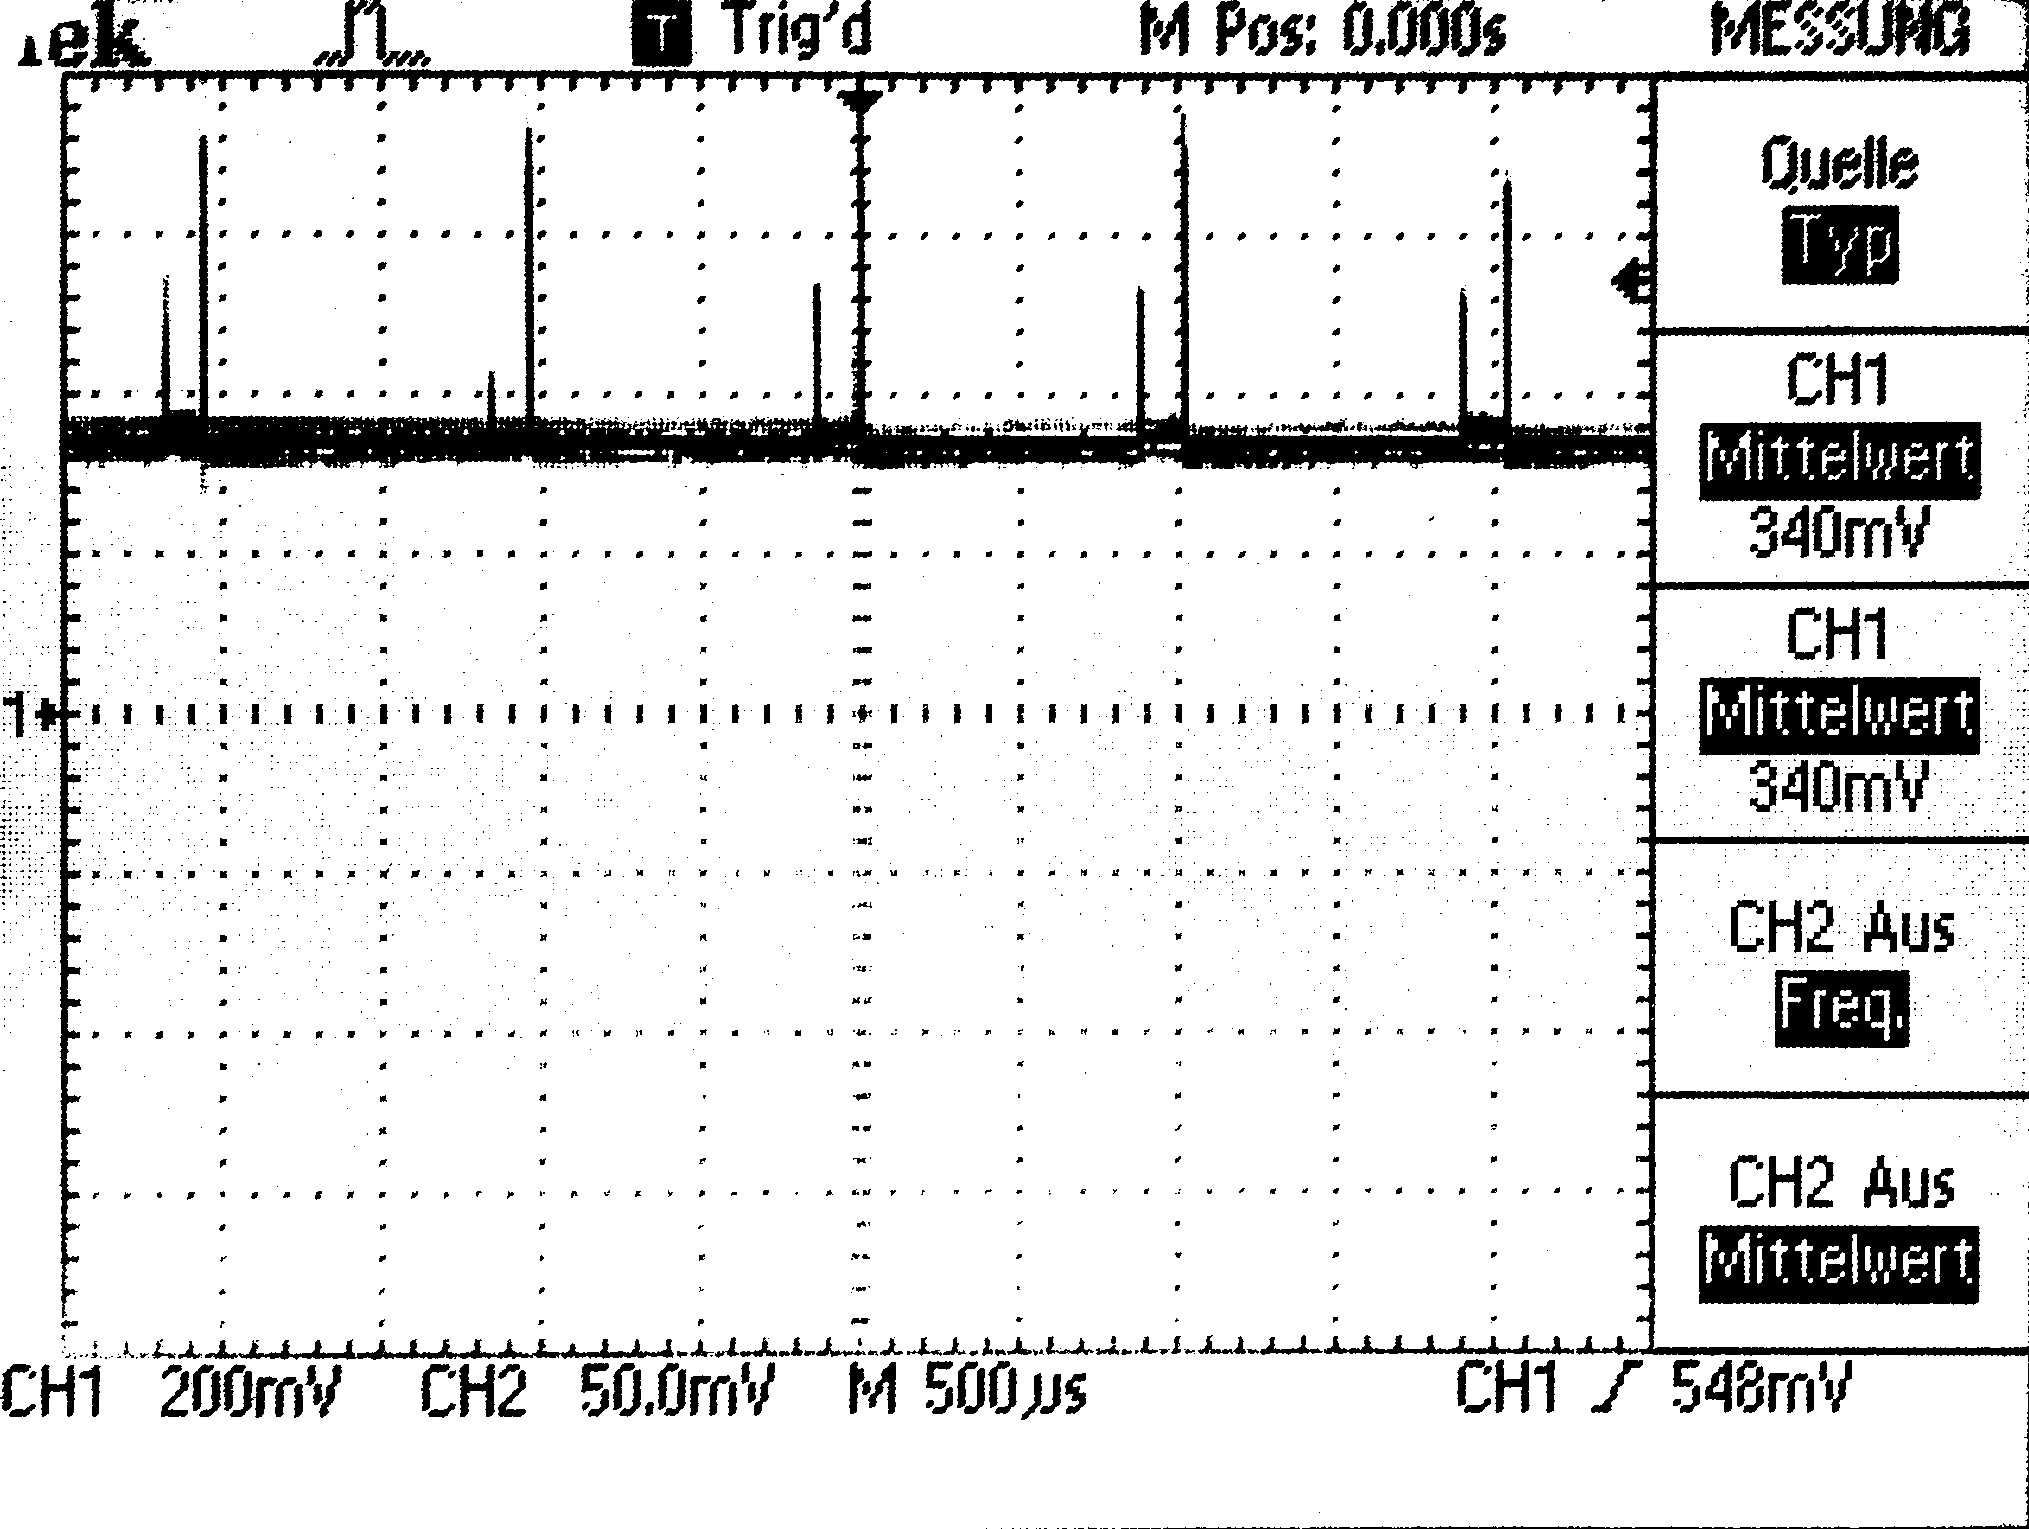
\includegraphics[width=.8\textwidth]{IR_spikes.png}\\
\caption{Ausgangssignal GP2D120}%
\label{fig:IR_spikes}
\end{figure}

Nach der Entstörung mit einem 82nF Kondensator direkt am Sensor zwischen VCC und GND sind die Störungen bereits stark vermindert.

\begin{figure}[H]
\centering
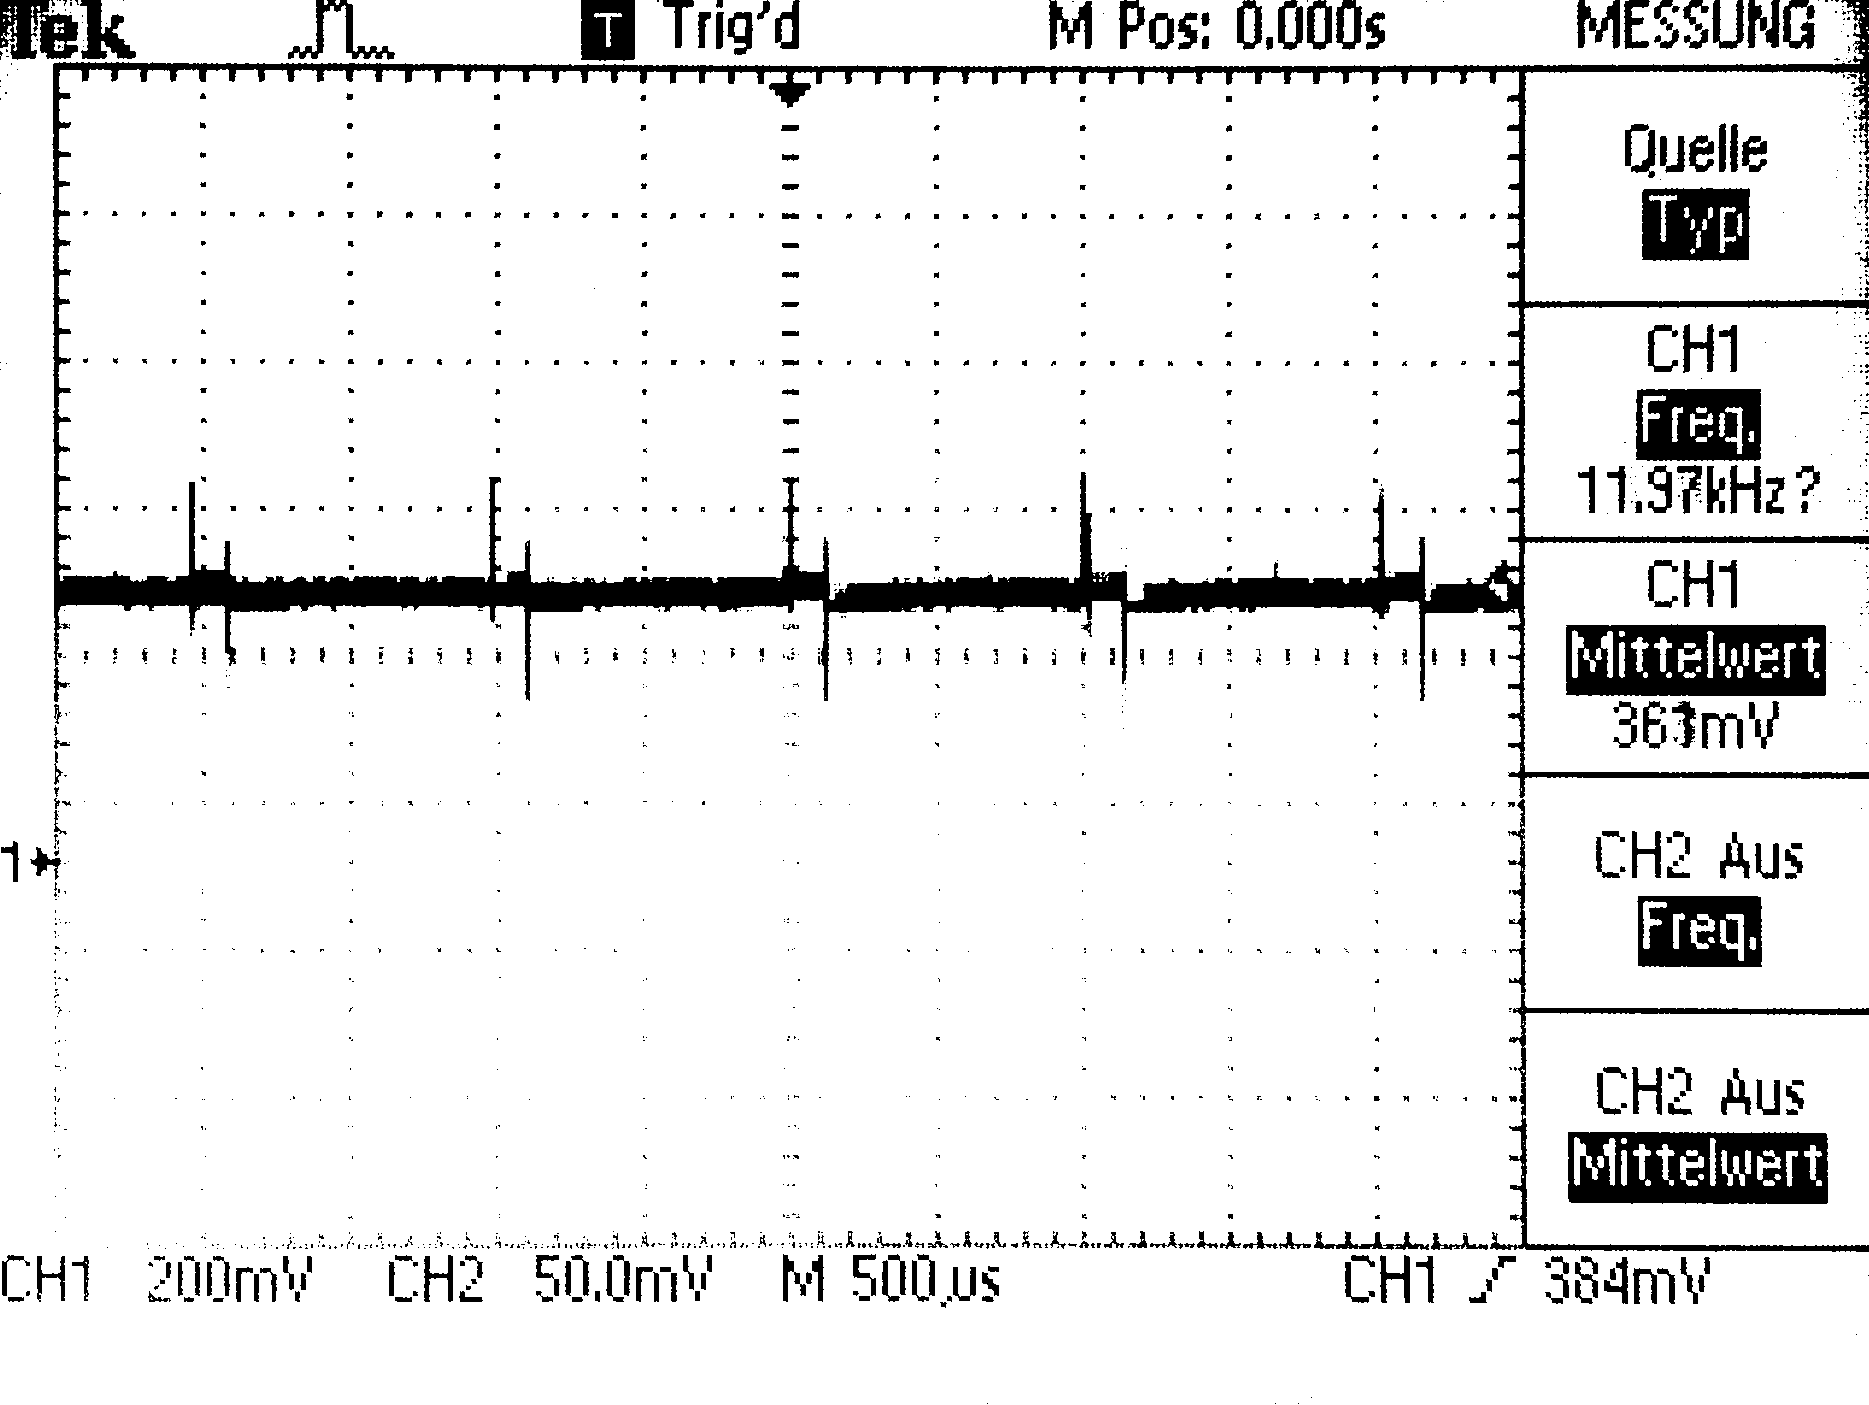
\includegraphics[width=.8\textwidth]{IR_lessspikes.png}\\
\caption{Ausgangssignal GP2D120 entstört}%
\label{fig:IR_lessspikes}
\end{figure}

\subsection{Auswertung des Messignales}
Das Messsignal vom Sensor wird über einen ADC-Eingang des AVR Microcontrollers ausgelesen. Angeschlossen werden die Sensoren über die PH-Connector Reihe des Herstellers JST, welche auch an den Sensoren verbaut sind.



\section{Odometrie}
Da Auto benötigt in unterschiedlichen Situationen unterschiedlich viel Leistung um seine Geschwindigkeit zu halten.
Besonders in Kurven ist durch die erhöte Reibung mehr Motorleistung nötig. Über den Motortreiber lässt sich jedoch nur
die mittlere Spannung am Motor verändern, deshalb ist es nötig diese zu regeln. Dafür ist jedoch eine Rückführung der Geschwindigkeit
des Autos nötig. Eine Aufintegrierung der Beschleunigungsdaten der Inertialsensorik führt auf Dauer leider zu erheblichen
Abweichungen und ist daher für eine Regelung nicht geeignet. Leider ist auch eine Odometrie an den Rädern des Autos
aus mechanischen Gründen schwer zu realisieren. 

Durch die feste Übersetzung des Getriebes bietet sich die Messung der Motordehzahl an. Damit lässt sich eine gute Nährung für die aktuelle Geschwindigkeit erreichen. 

\subsection{Hall-Sensor}
Eine Möglichkeit die Motordrehzahl zu messen ist es das Magnetfeld des
Motorankers auszuwerten. Dazu sehen wir uns den Aufabu eines Gleichstommotors an.
\begin{figure}[H]
\centering
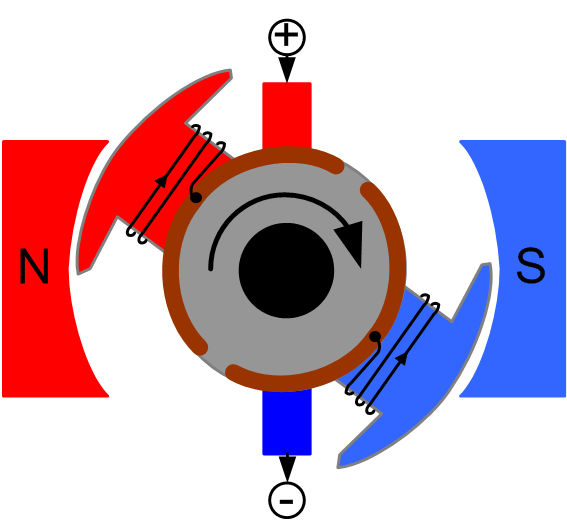
\includegraphics[width=.5\textwidth]{motor.png}\\
\caption{Aufbau eines Gleichstommotors \cite{gs-motor}}%
\label{fig:aufbau_motor}
\end{figure}
Ein Gleichstommotor besteht aus zwei grundsätzlichen Teilen, einem unbeweglichen Teil, den Stator und einem beweglichen Teil, dem Anker.
Der Stator besteht aus sich gegenüberliegenden Permanentmagneten welche zwei entgegengesetzt gepolte Magnetfelder erzeugen.
Der Anker besteht aus Elektromeganeten dessen Polung jede halbe Umdrehung kommutiert wird. Duch die Kommutierung ändert sich die 
Polung der Elektromeganeten. Das sich so änderne Magnetfeld kann mit einem Hallsensors ausgewertet werden. Das entstehende 
Signal ähnelt dabei über der Zeit einer Sinusschwigung. Mit Hilfe eines Schmitt-Trigger kann daraus ein Drehzahlsignal generiert werden.

Der Hallsensor ist erfolgreich durch ein Belüftungsloch im Motor plaziert wurden. Als Referenzspannung für den Schmitt-Trigger wird der
Mittelwert des Sensorsignals, erzeugt durch einen Tiefpass, genutzt.

\begin{figure}[H]
\centering
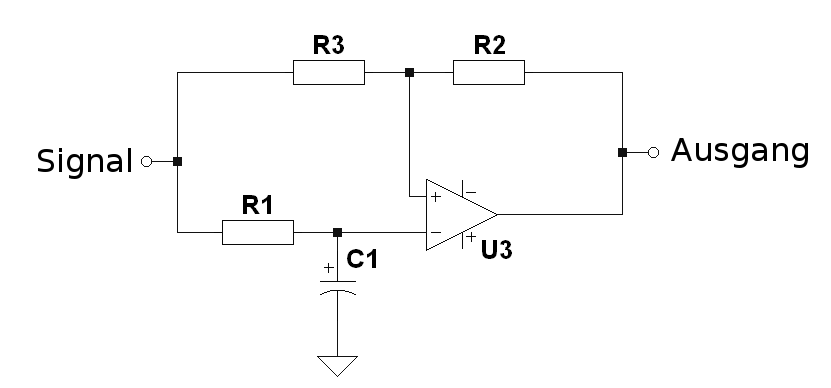
\includegraphics[width=.5\textwidth]{schmitt.png}\\
\caption{Schmitt-Trigger Schaltung}%
\label{fig:schmitt}
\end{figure}

Leider führt dieses Vorgehen nicht zum Erfolg, da die Magnetfeldstärke stark von der Drehrichtung des Motors abhängt. Es war nicht möglich
den Schmitt-Trigger so auszulegen, das er in beide Drehrichtungen zuverlässig funktioniert.

\subsection{Gabellichtschranke}

Alternativ zum Vorgehen mit einem Hall-Sensor wurde eine andere Lösung implementiert. An eine speziell für diesen Motor angefertigte Achsverlängerung wurde eine Inkrementalgeberscheibe befestigt, zu sehen in \cref{fig:gabellichtschranke}. 
Diese wird durch einen Sharp GP1A30R Sensor ausgewertet, welcher ein Drehszahlsignal an den externen Takteingang des Timer 1 vom AVR Microcontroller liefert.
\begin{figure}[H]
\centering
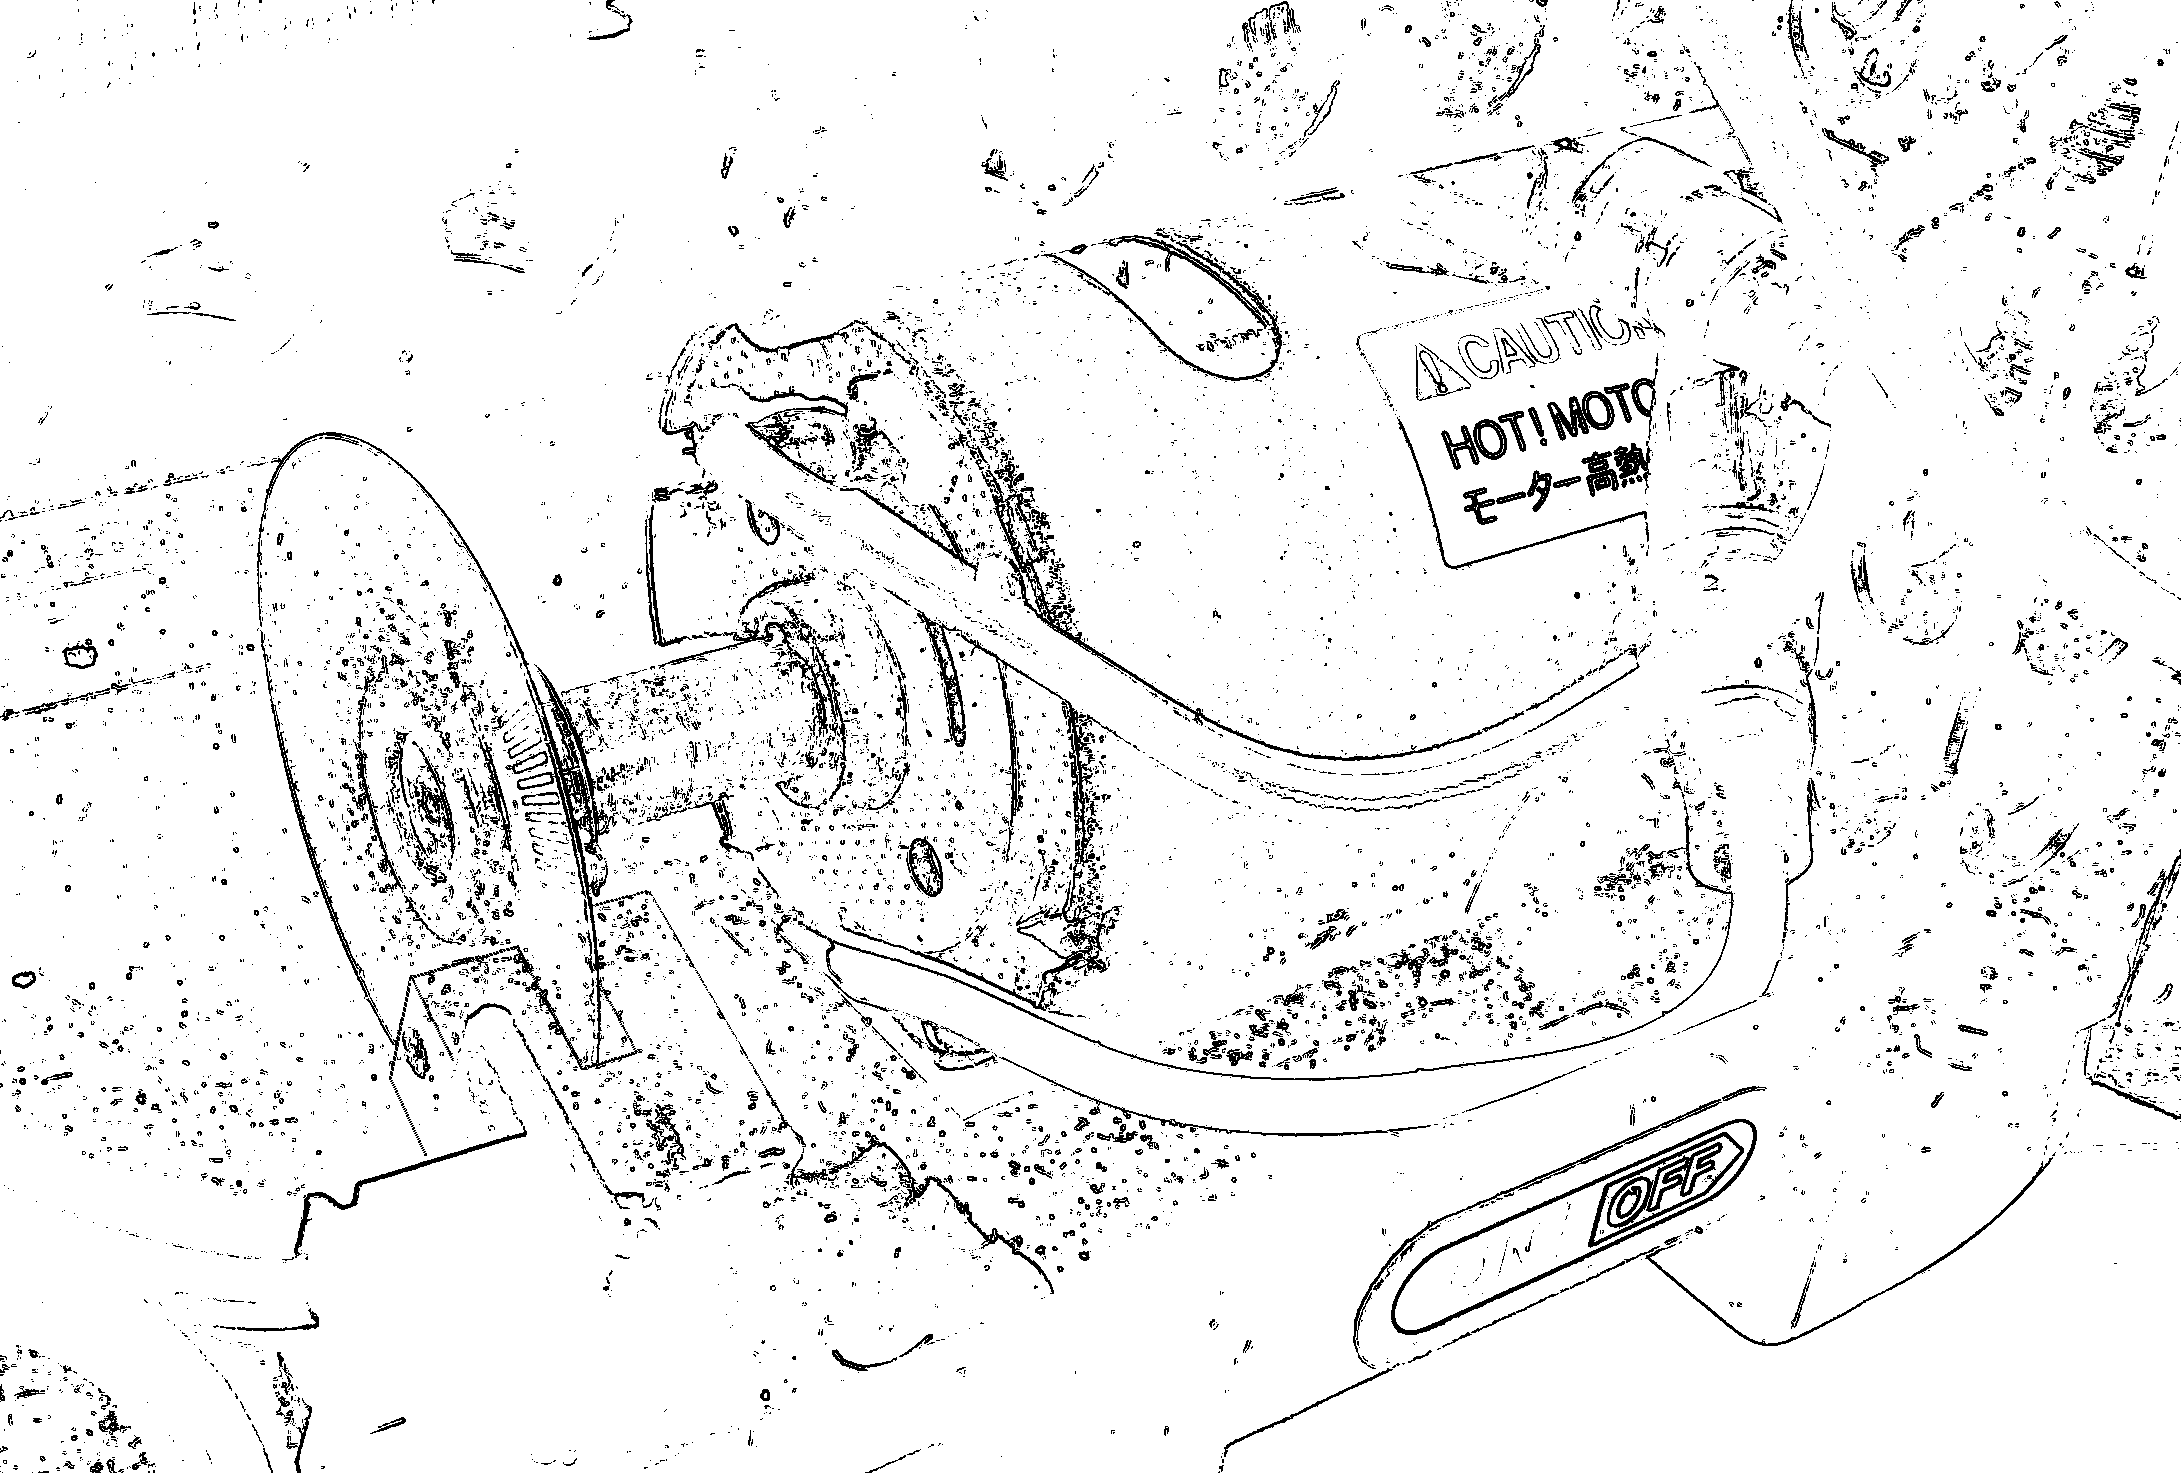
\includegraphics[width=.8\textwidth]{odometrie.png}\\
\caption{Motor mit Inkrementalgeber}%
\label{fig:gabellichtschranke}
\end{figure}

Die Scheibe ist dabei mit 120 Strichmakierungen versehen. Eine Motorumdrehung entspricht also 120 Impulsen, im folgenden Motorticks genannt. Über das Übersetzungsverhältnis des Getriebes und dem Radumfang kann dann 
der zurückgelegte Weg berechnet werden. Das Übersetzungsverhältnis des Fahrzeugs ist abhängig von drei Komponenten, dem Stirnrad, dem Motorritzel sowie einer festen internen Übersetzung. Das verwendtete Stirnrad hat
61 Zähne, das Motorrizel 19. Damit ergibt sich ein Verhältnis von 61:19 zusammen mit der internen Übersetzung von 2.6 \todo{Quelle raussuchen für interne Übersetzung} 
haben wir ein Übersetzungsverhältnis von 8,35. Der Radumfang beträgt ca. \SI{21}{\cm}.

\begin{align}
\frac{120*8,35}{0.21m}=\frac{ticks}{m}=4760
\end{align}

Mit dieser Größe lassen sich die Motorticks einfach in Meter umrechnen. 

\section{Auslegung der Stromversorgung}

Um das Layout der Platine möglichst simpel zu halten und damit kostengünstig zu bleiben, wurden alle Komponenten so ausgewählt, dass diese über eine einzige 5V Spannungsquelle mit Energie versorgt werden können.
Es ist wichtig den Stromverbrauch aller Komponenten abzuschätzten, um die Spannungsversorgung sinnvoll dimensionieren zu können. Eine zu schwache Spannungsquelle kann zu Instabilitäten führen,
während eine überdimmensionierte Geld verschenkt.

\subsection{Stromverbrauch der Komponenten}
In diesem Abschnitt soll eine Abschätzung des Stromverbrauches vorgenommen werden. Dabei wird keinen Wert auf hohe Genauigkeit gelegt, es soll nur eine ungefäre Größenordnung für den Stromverbrauch gefunden werden.

\subsubsection{Servomotor}-
Der Stromverbrauch des Servomotors ist schwer zu ermitteln. Da es sich um einen Modellbauservomotor handelt 
sind im Datenbatt hierzu leider keine Daten aufzufinden. Da ein Messaufbau für die Abschätzung des Stromverbrauches
zu aufwändig ist, werden hier Messwerte eines ähnlichen Servos aus einem Artikel \cite{website-servo} herangezogen.
Laut diesem hat eine Servomotor keinen konstanten Stromverbrauch. Der Srtomfluss wird immer wieder unterbrochen, so das es zu einem intervallartigen Stromfluss kommt.
Nur wenn der Servomotor dauerhaft belastet wird kommt es zu einem konstanten Stromfluss.
Im Artikel werden mehrere Servomotoren vermessen, der Motor der dem verwendeten am nächsten kommt ist der ``Graupner 4421'' mit folgenen Daten:

%TODO
\todo{Servo modell \cite{website-servo-dat} in Anforderungen mit aufnehmen}

Technische Daten ``Graupner 4421'' \cite{website-servo-vergleich-dat}:
\begin{itemize}
 \item Stellzeit(60°): 0,11s
 \item Stellmoment: 88Ncm 
\end{itemize}


Technische Daten des verwendeten Servomotors \cite{website-servo-dat}:
\begin{itemize}
 \item Stellzeit(60°): 0,13s (4,8V) / 0,16s (6,0V)
 \item Stellmoment: 92Ncm (4,8V) / 78Ncm (6,0V)
\end{itemize}



Dieser hat laut des Artikels eine maximale Stromaufnahme von 1,2A. Um noch Luft nach oben zu haben wird hier ein Verbrauch von 
1,8A angenommen.

\subsubsection{Pandaboard ES}
Leider gibt es vom Hersteller des Pandaboards keine konkreten Angaben zum Stromverbrauch. Der Hersteller empfiehlt jedoch ein
Netzteil mit 4A\cite{website-panda-supply}, wobei auch ein Betrieb an USB mit Hilfe eines Y-Kabels möglich ist. Die USB-2.0 Spezifikation\cite{website-usb-spec} sieht eine maximale 
Stromabgabe von 500mA vor.

Der Stromvebrauch des normalen Pandaboards (ohne ES) beträgt ca. 800mA \cite{website-panda-power}.
Nähere Angaben zu Stromverbrauch des normalen Pandaboards (ohne ES) finden sich in \cite{website-panda-power}.
Der Verbrauchdes Pandaboard ES dürfte durch den schnelleren Prozessor minimal darüber liegen. 
Durch Anschluss von USB-Geräten an das Board kann der Stomverbrauch jedoch noch steigen, Die USB-Spezifikation \cite{website-usb-spec}
sieht pro Port eine maximale Stomentnahme von 500mA vor. Da das Pandaboard über 2 USB-Ports verfügt liegt der maximale zusätzliche Verbrauch bei 1A,
so dass hier ein Gesammtverbrauch von 2A veranschlagt wird.

\paragraph{Hinweis:}
Das Pandaboard ES wurde im Laufe des Projekts durch einen Intel NUC ersetzt, welcher jedoch nicht über die 5V Schiene versorgt wird.
Daher entfällt der Verbrauch des Boards in den Messungen der Evaluierung.

\subsubsection{Led Beleuchtung}
Auch wenn LEDs den Ruf haben besonders energieffizient zu sein, ist der Stromverbrauch bei einer größeren Anzahl nicht zu
unterschätzen. Da wir RBG-LEDs einsetzen besteht ein LED-Modul aus 3 LEDs in den Grundfarben rot, blau und grün.
Laut Datenblatt \cite{ds-WS2812} haben die LEDs eine Stromaufnahme von 20mA, also 60mA pro Modul.
Um reglelwerkkonform zu sein, werden folgende Beleuchtungen benötigt: Blinker rechts und links jeweils vorne und hinten.
Sowie eine Leuchte, welche den RC-Modus anzeigt. Zusätzlich zu den im Reglelwerk vorgeschriebenen Beleuchtungen werden noch je
zwei Frontscheinwerfer und Rückleuchten integriert, so dass sich eine Anzahl von 9 LED-Modulen ergibt.
Der maximale durch die LEDs verursachte Strom liegt somit bei 540mA. 


\todo{Bremslichter???}


\subsubsection{Microkontroller}
Der maximale Stromverbrauch des AVR Mikrocontrollers liegt laut Datenblatt\cite{ds-at90can} bei 200mA, wenn IO-Pins belastet werden
Der Mikrocontrollers selber braucht jedoch bei 5V Betriebsspauung und 16MHz nur 29mA. Da die IO-Pins des Controllers nur wenig belastet werden,
wird hier nur ein Verbrauch von 100mA veranschlagt.

\subsubsection{Sharp Sensoren}
Die Sharp GP2D120 Distanzsensoren verbrauchen laut Datenblatt \cite{ds-sharp-GP2D120} 50mA, da zwei dieser Sensoren verbaut werden ergeben sich 100mA.

\subsubsection{Sonstige Peripherie}
Da der Stromverbrauch der restlichen Komponenten minimal ist werden hier pauschal 100mA veranschlagt.

\subsection{Auswahl des Reglers}
Der Gesamtstromverbrauch der Komponenten beträgt 4.740mA. Ein Linearregler ist hier nicht mehr praktikabel, da dieser bei einer Akkuspannung von 14,4V und 3.740mA fast 45 Watt Leistung in Wärme umwandeln würde.

\todo{verbessern..}
Eine gute Wahl für diesen Einsatzzweck ist der LM2678 von Texas Instruments, dieser kann dauerhaft einen Strom von 5A liefern und sein Wirkungsgrad liegt selbst bei Maximallast bei über 80\%.
Eine Übersicht dazu findet sich in Abbildung [\ref{fig:vreg-eff}].
\begin{figure}[H]
\centering
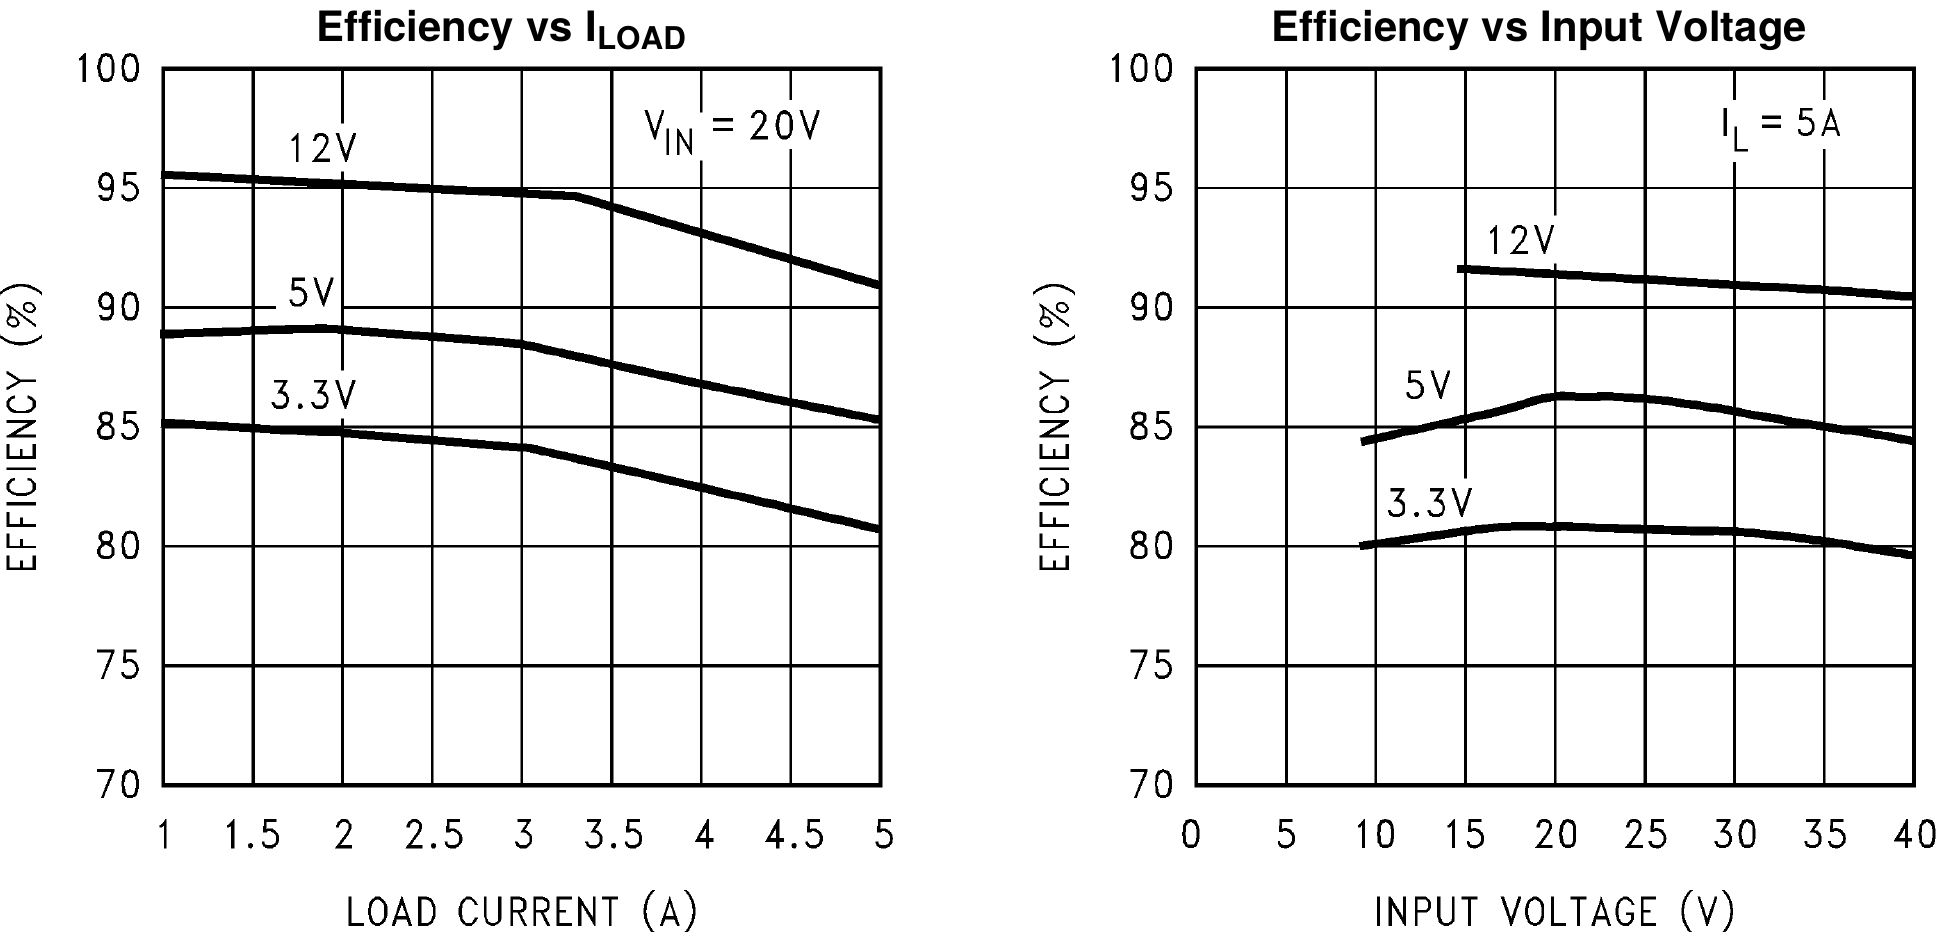
\includegraphics[width=.8\textwidth]{vreg.png}\\
\caption{Regulator Wirkungsgrad \cite{ds-ti}}%
\label{fig:vreg-eff}
\end{figure}
Ausgehend von ca. 24 Watt Leistungsaufnahme ($4,8A*5V$) und einem minimalen Wirkungsgrad von 80\%  ergibt sich damit eine überschauliche Verlustleistung von 6 Watt.


\begin{figure}[H]
\centering
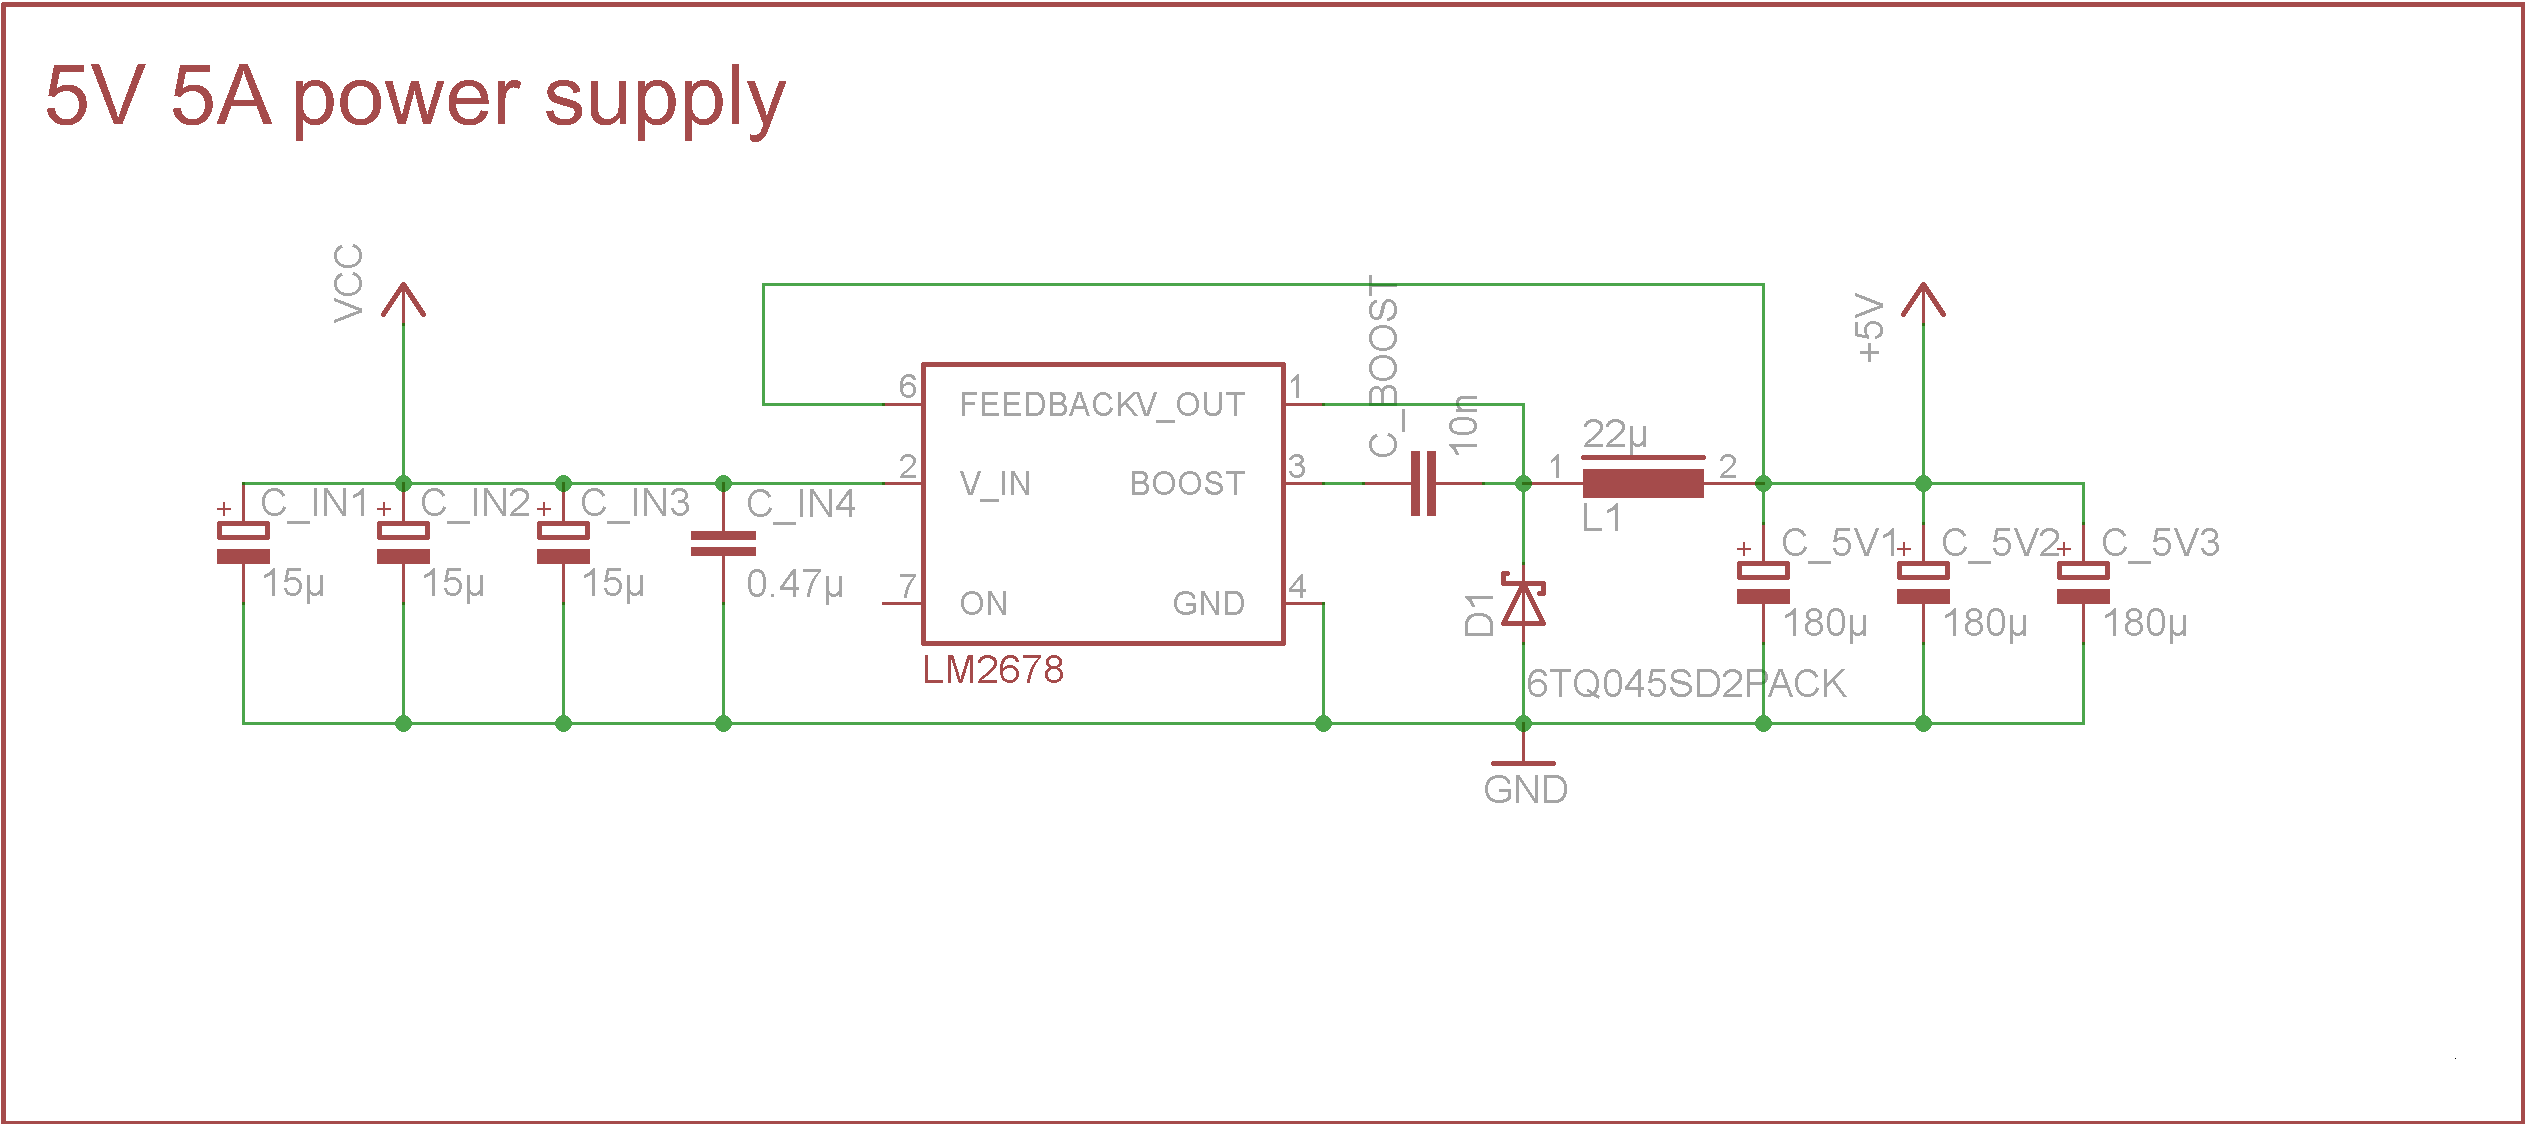
\includegraphics[width=.8\textwidth]{5vregler.png}\\
\caption{Schaltplan des 5V Reglers}%
\label{fig:vreg}
\end{figure}

\subsubsection{Low-ESR Kondensatoren}

Low-ESR Kondensatoren zeichen sich durch einen niedrigen Serienwiderstand ($R_{ESR}$) aus.
Dieser liegt in Reihe(Serie) zum idealen Kondensator (\cref{fig:esr}). 

\begin{figure}[H]
\centering
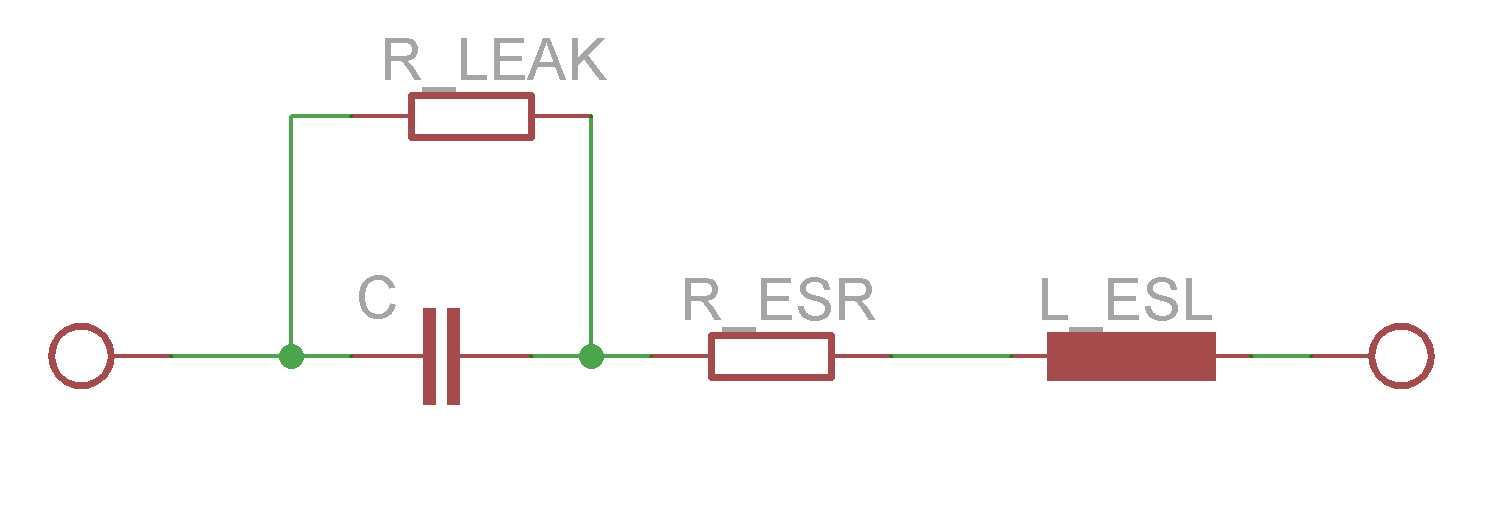
\includegraphics[width=.5\textwidth]{esr.png}\\
\caption{Ersatzschaltbild eines Kondensators}%
\label{fig:esr}
\end{figure}

Dieser verursacht Verluste innerhalb des Kondensators, was bei Belastung zur erwärmung des Kondensators führt und
seine Lebensdauer verringert. Desto kleiner der ESR desto niedriger die Verluste im Kondensator. Weiterhin
kann ein Kondensator mit kleinem ESR schneller ge- und entladen werden, als ein herkömmlicher Kondensator.
%Im entlade Fall kann man sich den Kondensator als Spannungsquelle vorstellen, der ESR stellt dann den Innenwiderstand der Spannungsquelle dar.
Durch diese Eigenschaft ist ein ESR Kondensator hervorragend zur Störunterdrückung geeignet.


Die Beschaltung erfolgt dabei nach den Empfehlungen des Datenblattes. Die verwendeten \SI{180}{\uF} Kondensatoren sollen laut Datenblatt low ESR Kondensatoren sein. Die verbauten Kondensatoren stammen aus Nichicons L8 Serie und haben einen Serienwiderstand von nur \SI{12}{\mohm}.

\section{Zusammenfassung}




\section{Software}

Die Software besteht im Grunde aus zwei Teilen, zum einem der Firmware auf dem Microcontroller zum anderem aus der Software auf der Recheneinheit, welche die Daten vom Microcontroller ausliest und über ROS publisht.
\todo{publisht oder published????????????}
In den folgenden Abschnitten werden erst die beiden Softwareteile erläutert, dann wird das Übertragungsprotokoll veranschaulicht.


\subsection{Software auf dem \textmu Controller}
Die Software auf dem Microcontroller ist vollständig in C++ geschrieben. Eine volständige Dokumentation der Software ist als Doxygen Dokument verfügbar. 
Die Software fungiert auf dem Controller als Service und wartet legendlich auf eine Anfrage von der seriellen Schnitstelle, welche sie bearbeitet und bei Bedarf beantwortet. 


\subsection{Client Programm auf der Recheneinheit}
Das Client Programm, im folgenden SerialNode genannt,
Im erten Schritt wurde hier ein Python Programm genutzt, welches jedoch einen Nachteil mit sich bringt. Da das Ansprechen der seriellen Schnitstelle unter pyserial sehr hohe CPU-Last mit sich bringt.
Da die so verschwendete Rechenleistung für andere Aufgaben benötigt wird und auch energieeffizienz ein wichtiges Kriterium ist, Wurde das Programm erneut in C++ implementiert. Unter verwendung der Systemaufrufe von 
Poll konnte das abfragen der seriellen Schnitstelle auf Systemebene ausgeführt werden, was die effizeinz stark verbessert. Während die Python Implementierung einen CPU-Kern zu 100\%
auslastete liegt die C++ Implementierung im unteren einstelligen Bereich.


 Das Programm stellt dann folgende Ros-Topics zur verfügung:\\
 
\begin{table}[H]
  \centering
  \begin{tabularx}{\textwidth}{|X|l|X|}
    \hline
     Ros-Topic 			& Ros-Datentyp		 	& Beschreibung 	\\ \hline \hline
    /sensors/current		& std\_msgs/Float32		& Der aktuelle Motorstom in Ampere								\\ \hline
    /sensors/imu/data\_raw	& ottocar\_msgs/simpleImu	& Die Daten werden im Standartformat für Inertialsensoren zur Verfügung gestellt		\\ \hline
    /sensors/IR1		& std\_msgs/Float32		& Der aktuelle Spannungswert des Sensors in Volt						\\ \hline
    /sensors/IR2		& std\_msgs/Float32		& Der aktuelle Spannungswert des Sensors in Volt						\\ \hline
    /sensors/motor\_revolutions	& std\_msgs/UInt32		& Die Anzahl der vergangenden Motorumdrehungen seit dem Start des Microcontrollers		\\ \hline
    /sensors/motor\_state	& std\_msgs/UInt8		& Der aktuelle Zustand des Motortreibers							\\ \hline
    /uC\_time			& std\_msgs/UInt32		& Die vergangende Zeit auf dem Microcontrollers seit dessen start in Millisekunden		\\ \hline
    /sensors/voltage		& std\_msgs/Float32		& Die aktuelle Akkuspannung in Volt								\\ \hline

  \end{tabularx}
  \caption{Ros-Publisher}%
  \label{tab:ros-pub}
\end{table}


 Das Programm hört auf folgende Ros-Topics:\\

\begin{table}[H]
  \centering
  \begin{tabularx}{\textwidth}{|X|l|X|}
    \hline
     Ros-Topic 			& Ros-Datentyp		 	& Beschreibung 	\\ \hline \hline
    /actuators/speed\_cmd		& std\_msgs/Int8		& Die neue Motorgeschwindigkeit von -128 bis +127		\\ \hline
    /actuators/angle\_cmd		& std\_msgs/Int8		& Der neue Servowinkel von -128 bis +127			\\ \hline
    /actuators/motor\_reset		& std\_msgs/Bool		& Initiiere einen Reset im Motortreiber				\\ \hline
  \end{tabularx}
  \caption{Ros-Subscriber}%
  \label{tab:ros-sub}
\end{table}



\subsection{Übertragungsprotokoll}
Da die Übertragung der Daten via ROS-Serial im ersten Prototypen zu vielen Problemen geführt hat, wurde ein neues Übertragungsprotokoll entwickelt.
Dabei wurde auf Fehlertoleranz und niedrigen Ressourcenverbrauch geachtet. Der Datendurchsatz muss hier ausreichend sein um alle Daten stabil mit 100Hz
übertragen zu können.
Der Grundlegende Ablauf der Datenübertragung ist in den Abbildungen [\ref{fig:uC_read}] und [\ref{fig:uC_write}] zu sehen.

\todo{in Bildern NUC duch recheneinheit ersetzten??}

Während eines Lesevorganges wartet der Microcontroller auf ein fest definiertes Startsignal von der Recheneinheit. Nachdem das Startsignal empfangen wurde, wird auf eine weitere Preamble gewartet.
Dies ist notwendig um bei Asynchronitäten die Wahrscheinlichkeit eines zufälligen Startsignals zu verringern. Wurde die Preamble erfolgreich empfangen erwartet der Microcontroller eine gültige Topic ID.
Wurde eine falsche Preamble empfangen wartet der Microcontroller erneut auf ein gültiges Startsignal. Abhängig von der Topic ID verfährt der Microcontroller dann im Programm fort und beantwortet
die Anfrage entsprechend. Für manche Topics ist eine Bestätigung (Acknowledge) nötig. Bekommt der Microcontroller keine Bestätigung sendet er die Daten erneut. Eine Bestätigung wird nur gesendet,
wenn die vom Client berechnete Checksumme mit der mitgesendeten identisch ist. Dies ist besonders bei den Daten der Inertialsensorik von nöten, da hier defekte Daten zu einem dauerhaften Fehler führen. 
Die Anzahl dieser Retransmits ist begrenzt und wird vom Client festgelegt. Wurde ein Acknowledge empfangen oder für den Topic ist keine Bestätigung
nötig, wartet der Controller erneut auf ein Startsignal.

\begin{figure}[ht]
\centering
\includegraphics[page=1,width=.8\textwidth]{graph/read.pdf} 
\caption{Lese Daten}
\label{fig:uC_read}
\end{figure}

Der Ablauf eines Schreibvorganges auf dem Microcontroller ist ähnlich. Der Microcontroller wartet auf das Startsignal und eine Preamble sowie eine Topic ID.
Nach dem Empfang der TopicID erwartet er die nötigen Daten, samt Checksumme. Diese ist nötig um die Daten zu verifizieren. Bei der Ansteuerung des Motors kann ein
Bitfehler zu fatalen Folgen führen. Beispielsweise kann die Recheneinheit oder der Microcontroller abstürzen wenn die Motorleistung plötzlich stark erhöt wird.
Daher werden die Daten nur übernommen, wenn die Checksumme erfolgreich verifiziert wurde. Sollte die Checksumme nicht verifiziert werden, springt der Microcontroller
erneut in des Startzustand und wartet auf ein Startsignal, ohne die Daten zu übernehmen. Der Client bekommt davon nichts mit, wenige einzelne Fehler können durch die
hohe interne Datenrate von 100Hz ignoriert werden. Haufige oder dauerhafte Fehlübertragungen, können durch die Reaktion des Autos leicht identifiziert werden.
Häufige oder dauerhafte Fehlübertragungen würden duch das fortlaufende Lesen und Schreiben auf dem Microcontroller so oder so zu Fehlern in beiden Richtungen führen.

\begin{figure}[ht]
\centering
\includegraphics[page=1,width=.8\textwidth]{graph/write.pdf} 
\caption{Schreibe Daten}
\label{fig:uC_write}
\end{figure}





